\documentclass[12pt,onecolumn]{revtex4-2}    % Font size (10,11 or 12pt) and column number (one or two).


\usepackage{times}                          % Times New Roman font type
\usepackage{float}
\usepackage{booktabs}
\usepackage{amsfonts}
\usepackage{subcaption}
\usepackage{gensymb}

\usepackage[a4paper, left=2.5cm, right=2.5cm,top=2.5cm, bottom=2.5cm]{geometry}       % Defines paper size and margin length, 1.85 for all
\renewcommand{\baselinestretch}{1}

\usepackage[font=small, labelfont=bf]{caption}                      % Defines caption font size as 9pt and caption title bolded


\usepackage{graphics,graphicx,epsfig,ulem}	% Makes sure all graphics works
\usepackage{amsmath} 						% Adds mathematical features for equations

\usepackage{etoolbox}                       % Customise date to preferred format
\captionsetup{justification=raggedright,singlelinecheck=false}

\makeatletter
\patchcmd{\frontmatter@RRAP@format}{(}{}{}{}
\patchcmd{\frontmatter@RRAP@format}{)}{}{}{}
\renewcommand\Dated@name{}
\makeatother

\usepackage{fancyhdr}


\pagestyle{fancy}                           % Insert header
\fancyhead{} % clear all header fields
\fancyhead[L]{\fontsize{10}{12} \selectfont Rebecca J. Hedley}
\fancyhead[R]{\fontsize{10}{12}
\selectfont The Martian Climate: past and present}

%\renewcommand{\headrulewidth}{0pt}
%\lhead{Rebecca J. Hedley}                          % Your name
%\rhead{Replicating Mars' Climate: Applying a 1-Dimensional Energy Balance Climate Model}            % Your report title               

\def\bibsection{\section*{References}}        % Position reference section correctly
\bibliographystyle{plain}

%%%%% Document %%%%%    
\begin{document}


\title{The Martian Climate: past and present} 
\date{Submitted: \today{}}
\author{Rebecca J. Hedley}
\affiliation{\normalfont Level 4 Project, MPhys Physics\\ Supervisor: Drs. Richard Wilman and Craig Testrow\\ Department of Physics, Durham University}


\begin{abstract}              

Mars presents a complex case study of climate change given its history as a periodically warm and wet planet, with applications to astrobiology and understanding greenhouse feedback mechanisms on Earth. A one-dimensional energy balance model (EBM) is built using the finite difference method, based on a differential equation encompassing the effects of heat capacity, solar insolation, albedo, meridional heat diffusion, and outgoing radiation. Mean annual temperature values agree to a latitudinally averaged value of 1\% to Earth climate fit from literature, and to within 3.2\% when the same model is applied to Mars. Seasonal variations are clearly observed in the model and replicate more extreme variations expected on Mars, as well as the combined effects of obliquity and an eccentric orbit. Further work involving $\mathrm{CO_2}$ cycle modelling is discussed to improve the Mars model given the importance of the annual pressure cycle.

\end{abstract}

\maketitle

\thispagestyle{plain} % produces page number for front page

\newpage

\tableofcontents

\newpage

\section{Introduction} 

\subsection{Is There Life on Mars?}

There exists, as of yet, no evidence to indicate present-day organic life on Mars. However, by studying and modelling the climate of the red planet, we can make preliminary insights into whether Mars could have, or can in the future, host life. Appropriate conditions for liquid water are widely used as the basic criteria for a habitable planet, given that all life observed on Earth requires water for survival - while this might exclude a lot of species which don't rely on water for survival, the abundance of water in the solar system (and, in the past, on Mars) suggests this is a perfectly reasonable and non-restrictive condition for potential Martian life. It's possible that ancient Mars had an abundance of liquid water, and therefore maybe an abundance of life.

\

Temperatures close to both freezing and boiling point may seem too broad, however, extremophiles are capable of existing under such conditions. Microorganisms isolated on Earth have displayed the ability to thrive at low temperatures, and even in simulated Martian environments: \textit{H. hispanica} and \textit{G. thermantarcticus} are just two extremophiles that resisted days of Martian temperatures and pressures in lab conditions \cite{M14}.

\

Dimensionally resolved climate models allow us to more fully understand the habitability of a planet. Zero-dimensional models only convey the most basic information about the energy balance of a planet, and so discount more complex climates which may sustain habitable environments at particular locations and uninhabitable conditions elsewhere. By the seemingly broad liquid-water definition of habitability, even the Earth is only partially habitable, and a zero-dimensional model would paint a much less comprehensive overview of Earth's climate. One-dimensional EBMs are therefore important to be able to assess temperatures at various latitudes and points in orbit, to provide the fullest chance of Mars having supported life in its history.

\

Additionally, the study of Mars' climate allows insight into climate change mechanisms. It is clear that human activity is capable of globally changing the environment, and it is strongly suggested that action is taken to prevent any further warming \cite{IPCC23}. The process of developing accurate climate models aids this purpose, in addition to exploring the efficiency of warming and cooling mechanisms for application to the Earth.

\subsection{Martian History}
%Milakovitch cycles
%pressure cycles
%current climate
%ancient climate

Martian history is generally split into the following three time periods, each characterised by severely differing climates. Modern-day Mars (known as the Amazonian period), between 0 - 3.0 Ga ago, is epitomised by dry and cold conditions, and a thin (95\% $\mathrm{CO_2}$) atmosphere which is, on average, less than 1\% of Earth's surface pressure. The climate is largely influenced by the behaviour of the $\mathrm{CO_2}$ atmosphere in daily and annual cycles, with mean surface pressure varying by up to 30\% seasonally. This is as a result of the condensation of $\mathrm{CO_2}$ at each pole during the winter; the ice caps grow by between 1.5-2m from summer to winter (on top of residual $\mathrm{H_2O}$ caps, which are permanent features of both poles). This change is large enough to cause a measurable change in Mars' gravitational field. The condensation-sublimation cycle of $\mathrm{CO_2}$ fixes the temperature of the poles to the freezing point of $\mathrm{CO_2}$, and forbids the temperature to drop below it.

\

In addition to the Martian pressure cycle, dust storms are one of the most significant influencing factors on the climate. Often the result of radiative heating, dust storms most commonly are observed between $L_{s}$ ~ 130-305$\degree$, encompassing the Southern spring equinox and summer solstice. The near-concurrence of the Southern summer solstice with the perihelion of Mars' present-day orbit is thought to further drive dust storms by creating a larger temperature gradient. It isn't uncommon for dust storms to reach regional ($\textgreater$ 1$\times 10^{7}$ $km^{2}$) or global scales and last anywhere between several days and several months - unsurprisingly, these storms significantly impact global heat retention \cite{WR13}. Large increases in opacity result in increases in temperature by up to 30K (observed in a regional storm during MY33, and also during the 2001 global dust storm). Global dust storms occur with a probability of approximately a third each year, however large regional storms occur reliably multiple times a year \cite{W20}.

\

The Hesperian era (3.0-3.5Ga) was characterised similarly by a warmer climate, and also by extensive volcanic activity. Sulfate deposits are found most commonly on terrain dated to this period, indicating volcanic sources, suggesting the presence of sulfur-bearing gases such as $\mathrm{SO_2}$ and $\mathrm{H_2 S}$ \cite{HKP02}. Such gases act as effective greenhouse gases, especially $\mathrm{SO_2}$, which absorbs far enough from the $\mathrm{CO_2}$ peak to potentially have caused a significant reduction in outgoing longwave radiation during this period \cite{HZS07}. It's possible that the addition of these greenhouse gases is the reason behind flooding events associated with the Hesperian era: large flood basalts and outflow channels indicate extreme volumes of meltwater \cite{HH14}. The Hesperian period is a transitory one, where the warm and wet climate of the Noachian era progresses into the arid Mars observed today.

\

\begin{figure}[b]
%\centering
\centering
\includegraphics[width = 15cm]{valleys.png}
\caption{Automated (orange lines )and manual mapping (blue lines) detection of valleys on the Martian surface in IR at a) Apollinaris Patera, shield volcano in the South, and b) valleys located around 48$\degree$E and 9$\degree$N. \cite{HBH10}}
\label{fig:valleys}
\end{figure}

The Noachian era (3.5-4.1Ga) was likely the wettest period in Mars' history. As a result of its absence of plate tectonics, an ecosystem, or global oceans, the Martian surface is preserved well enough for study of eras as early as this. Branching tributaries beginning near geographic peaks indicate precipitation, and the large valley networks these create are expected to have formed over timescales of $10^{5}$ - $10^{7}$ years, indicating a consistently active water cycle \cite{W16}. There is abundant evidence for crater lakes linked with larger valley networks, found most commonly in the Noachian southern highlands \cite{FH08}. Such valley networks can be seen in Fig. \ref{fig:valleys}. More controversially, it's even possible that a shallow ocean covered the Northern hemisphere of Mars \cite{H99}, although given that suggested shorelines vary by several kilometres it is unlikely. The geochemistry of Mars also points towards a hydrologically active planet - aluminium-rich clays, and aqueous minerals like chlorides, silicas, sulphates (which require water to form) and phyllosilicates are abundant in Noachian geology \cite{EE14}. 

\

However, low chemical alteration of the surface by water in lakes indicates that the streams responsible for these hydrological features were brief \cite{W13}. While there is much evidence for Noachian crater lakes, closed-basin lakes (from which water does not escape) outnumber open-basin lakes (from which water does escape, often to a larger lake or an ocean) which indicates a limited water inventory \cite{BHM09}. The geochemistry of Mars is promising, yet carbonates, which form readily on warm and wet surfaces, are almost absent \cite{C13} \cite{EE14}. Additionally, the presence of phyllosilicates can be explained by subsurface formation in water-poor systems \cite{E11}, further complicating interpretations of the evidence available. The only solid conclusion to draw from this array of evidence is that the hydrological cycle of Mars was a complex one, most likely a result of an intermittent water cycle. Still, the warming mechanism to allow episodic warm and wet periods is unclear.

\

The mystery of Mars' hydrological cycle deepens when the luminosity of the early Sun is considered. The "faint young Sun" paradox describes how the Sun's luminosity during the Noachian era was 75\% of its current value \cite{G81}, and given that its semi-major axis has not changed, there must have been some warming mechanism to achieve T \textgreater 273K. The possibility of the Sun shedding extra mass early on and providing a larger luminosity than expected has been considered, however, there is no evidence to support this anomalous behaviour other than its convenience for warming Mars \cite{MM07}. The obvious option is to generate a greenhouse effect via the inclusion of a much denser early $\mathrm{CO_2}$ atmosphere, which will be the warming mechanism explored in this work. The role of the Milankovitch cycles are also investigated.

\subsection{Climate Modelling}

\subsubsection{Energy Balance Models}
%"habitable climates" has some good info
Energy balance models predict global temperatures by a radiative energy budget, estimating energy received from the Sun and energy retained or reflected by the planet. The most simple EBM is the zero-dimensional case, a model which predicts a single mean surface temperature to the whole planet by assuming that the energy received is equal to the energy lost in a steady state solution. The 0D EBM neglects varying land distributions (and therefore temperature-dependent heat capacities, albedo values, and outgoing radiation) and heat diffusion between latitudes. They can provide relatively accurate estimates for global mean temperature \cite{L20}, however they cannot provide temperature as a function of latitude, and so are not appropriate for this study of Mars' climate.
\

One-dimensional EBMs, such as the model used in this study, split the planet into latitude bands and assess the temperature of each based on local variables such as solar insolation and ice distribution. 1D EBMs most importantly allow for meridional heat transport, an important factor in the local latitudinal energy budget for planets with a thick enough atmosphere \cite{SMS08}, and therefore important for the Earth validation study and later, for Mars'. As a result of the inclusion of heat diffusion, it is possible that each region at any particular time will not locally satisfy the energy budget condition Eq. 1. This is also possible for the planet as a whole on any day, especially due to an eccentric orbit. %Deviations from the energy budget are what create...

\subsubsection{General Circulation Models}

General circulation models (GCMs) are more complex three- (or four-) dimensional climate models which are based on fluid equations. Earth is split into horizontal grid cells longitudinally and latitudinally, and also split vertically based on height from surface or pressure. Processes which apply on scales smaller than that of the resolution of the grid, such as ice-albedo feedback or cloud effects on radiative flux, are parametrised, and these parametrisations create the largest source of error within a GCM \cite{CBZH}. Despite this, GCMs remain the most accurate computational representations of climate.
\

GCMs have had success modelling the $\mathrm{CO_2}$ cycle on Mars. Unlike EBMs, which assume $\mathrm{CO_2}$ condenses directly on the surface, GCMs allow for $\mathrm{CO_2}$ condensing in the atmosphere. Atmospheric $\mathrm{CO_2}$ behaves much differently to ice cap $\mathrm{CO_2}$ in that, whereas ice deposits are effectively transparent at infrared wavelengths, atmospheric $\mathrm{CO_2}$ particles efficiently scatter heat and therefore contribute to global cooling. Such effects on Mars have been observed to decrease total polar condensation rates by 10 - 20\% during the winter \cite{FP96}, therefore also affecting ice-albedo feedback and decreasing heat diffusion due to a reduced atmosphere. 
 
\section{Development of the Earth Validation Model} 
\subsection{Atmospheric Diffusion Differential Equation}
The differential equation which underpins the one-dimensional model is as follows:

\begin{equation}
C \frac{\partial T}{\partial t} = S(1-A) + \frac{\partial}{\partial x} [D(1-x^{2})\frac{\partial T}{\partial x}] - I.
\end{equation}

It concerns the proportion of incoming flux retained by the planet, represented by the first term $S(1 - A)$, outgoing flux represented by the last term $I$, and diffusive processes represented by the remaining middle term. The balance of these terms on the right hand side determines the change in temperature per timestep, $\frac{\partial T}{\partial t}$, on the left. It is possible, by a change of variable from $x$ to $\lambda$, to express this in terms of latitude,
\begin{equation}
C \frac{\partial T}{\partial t} = S(1-A) + D\frac{\partial^2 T}{\partial t^2} - D\tan\lambda\frac{\partial T}{\partial \lambda} - I,
\end{equation}
which is the expression used in the final computational model, where $C$ is heat capacity, $S$ is the daily averaged solar insolation, $A$ is the albedo, $D$ is the diffusion coefficient, and $x$ $\equiv \sin\lambda$ is the sine of the latitude.

The prescriptions for each of these terms are first developed to represent Earth's climate. The value of heat capacity is determined by the distribution of land, ocean, and ice (each with a different value of $C$). Uniform land/ocean distribution (30\% land, 70\% ocean) is assumed in every latitude band, and the proportion of ocean which is covered by ice is determined by the temperature at that band - bands below 263K are completely ice-covered, bands between 263-273K are partially ice-covered, smoothly increasing oceanic ice fraction $f_{ice}$,

\begin{equation}
f_{ice} = 1 - e^{\frac{T-273}{10}},
\end{equation}

as the temperature drops, and bands above 273K are ice-free. Prescribed heat capacities are as follows: $C_{land}$ = 5.25 $\times 10^{6}$ $\mathrm{Jm^{-2}K^{-1}}$, $C_{ocean}$ = 40 $C_{land}$, $C_{ice}$ = 9.2$C_{land}$ when 263K $< T <$ 273K, and $C_{ice}$ = 2.0$C_{land}$ when $T \le$ 263K. This is what makes the snowball transition almost impossible to transition out of - retained heat is reduced to approximately 30\% of the incoming value by a large albedo, and a larger heat capacity for ice, meaning melting ice requires heat transport from warmer latitudes. This is not viable on an ice-covered planet. As discussed above, S varies with latitude given its dependence on the solar zenith angle, and A similarly depends on the land, ocean, and ice distribution. 
\

$D$ is a function of atmospheric pressure $p$, atmospheric heat capacity $c_{p}$, rotation rate $\Omega$, and mean molecular weight of the atmosphere $m$. $D_{0}$ denotes the diffusion coefficient value for Earth, taken to be 5.394 $\times 10^{-1}$ $\mathrm{J m^{-2} s^{-1} K^{-1}}$, and similarly for other values the subscript 0 denotes the Earth value - $p_{0}$ = 1 atm by definition, $c_{p_{0}}$ = 1000 $\mathrm{g^{-1}K^{-1}}$, $m_{0}$ = 28, and $\Omega_{0}$ = 7.27 $\mathrm{rad s^{-1}}$.

\begin{equation}
\frac{D}{D_{0}} = \frac{p}{p_{0}} \frac{c_{p}}{c_{p_{0}}} {\frac{m_{0}}{m}}^{2} {\frac{\Omega_{0}}{\Omega}}^{2}
\end{equation}

For the Earth validation model, D is a constant since we don't consider pressure variations. Such variations will become important when modelling Mars' climate given the severe seasonal $\mathrm{CO_2}$ pressure changes of around 30\% annually \cite{FHT98}.

\subsubsection{Incoming Flux}

Total solar flux in each latitude band is proportional to the cosine of solar zenith angle $z$, which is expressed  as a function of latitude $\theta$, solar hour angle $h$, and solar declination $\delta$:

\begin{equation}
\cos z = \sin \theta \sin \delta + \cos \theta \cos \delta \cos h.
\end{equation}

The declination angle is a sinusoidal function dependent on orbital longitude and obliquity $\delta_{0}$, which reaches its extrema at the solstices. Solar hour angle describes the angular displacement of the Sun in a planet's sky from the meridian, and is zero degrees at noon. 
\
In order to find a diurnally averaged value for incoming solar flux, the cosine of solar zenith angle $z$ must be averaged over one rotation. First it is averaged over solar hour angle $h$ = - $H$ to + $H$, with H as radian half-day length,

\begin{equation}
H = \arccos(-\tan \theta \tan \delta),
\end{equation}

which corresponds to the fraction of a day during which the sun is above the horizon. 
\begin{equation}
\overline{\cos z} = \frac{\int_{-H}^{H} \sin\theta \sin\delta + \cos\theta \cos\delta \cosh dh}{\int_{-H}^{H} dh}
= \sin\theta \sin \delta + \cos\theta \cos\delta \frac{\sin H}{H}.
\end{equation}

If, during summers at the poles for example, the sun remains above the horizon for a complete day then $H$ = $\pi$ according to the above definition. At latitudes where the Sun remains in the sky for a fraction of a rotation, the average $\overline{\cos z}$ must be scaled then by $\frac{H}{\pi}$. In order to generalise to any planet with semimajor axis $a$ in AU, Eq. 4 is also scaled by a $\frac{1}{a^{2}}$ term. Multiplying by these factors and also by solar constant $q$, we find diurnally averaged incident solar flux $S_{0}$,

\begin{equation}
S_{0} = \frac{q}{\pi}(\frac{1.0 AU}{a})^{2}(H\sin \theta \sin \delta + \cos \theta \cos \delta \sin H).
\end{equation}

As of yet, we have assumed a circular orbit.
Total insolation received by a planet at a given time is a function of the position in its orbit (given that the orbit is not perfectly circular), and the solar zenith angle at each latitude. The instantaneous Sun-planet distance is given by the following expression,

\begin{equation}
r = \frac{a(1-e^{2})}{1 + e \cos \theta}
\end{equation}

where $e$ is the eccentricity of the orbit, $a$ is its semimajor axis, and $\theta$ is the true anomaly, an angular quantity which defines the position of a body in its orbit in respect to its periapsis. From the instantaneous position $r$ we can then include the effect of eccentricity on daily insolation by invoking the inverse square law,

\begin{equation}
S_{eccentric} = \frac{S_{0}}{r^{2}},
\end{equation}

where $S_{0}$ is the original expression Eq. 5 derived for a body with zero orbital eccentricity.

\subsubsection{Outgoing Flux}

Three prescriptions were tested for infrared cooling and albedo functions. The first two assume that the planet is a blackbody and therefore radiates energy proportional to $T^{4}$, which is then reduced through an optically thick atmosphere which reradiates heat back to the planet. The two models differ in that the second has a temperature dependent optical thickness, $\tau_{IR}(T)$, which acts to decrease infrared radiation escaping the atmosphere as the surface temperature increases. This reflects the temperature-dependent greenhouse effect, in which heat retention scales with the amount of water vapour in the atmosphere due to absorption. The third model is a simple linear relation obtained by applying a least squares fit to outgoing infrared flux data from satellite observations. The $\tau_{IR}$ models are borrowed from SMS08 \cite{SMS08}, and the linear model is borrowed from NC79 \cite{NC79}. These are outlined in Table I. 
\\
\begin{table}
\begin{tabular}{ccc} \toprule
    Model & IR Cooling Function & Albedo Function \\ \midrule
    1  & $I(T) = \frac{\sigma T^{4}}{1+ \frac{3}{4}\tau_{IR}^{0}}$ & $A(T) = 0.5 - 0.2 \tanh \frac{T - 268}{5}$ \\
    2  & $I(T) = \frac{\sigma T^{4}}{1+ \frac{3}{4}\tau_{IR}(T)}$  & $A(T) = 0.525 - 0.245 \tanh \frac{T - 268}{5}$ \\
    3  & $I(T) = A + BT $  & $A(T) = 0.475 - 0.225 \tanh \frac{T - 268}{5}$ \\
\bottomrule
\end{tabular}
\caption{Model 1 has fixed optical thickness $\tau_{IR}^{0}$ = 1. Model 2 has temperature dependent optical thickness $\tau_{IR}(T) = 0.79(T/273)^{3}$. Model 3 has constants A = 2.033 $\times 10^{2} Jm^{-2}s^{-1}$, B = 2.094 $J m^{-2} s^{-1} K^{-1}$}.
\end{table}

Albedo is dependent on fractional ice and snow cover, so varies according to temperature. In each formulation, surface albedo is parametrised to be between 0.25-0.3 for ice-free surfaces above 273K, and 0.7-0.77 for ice-covered surfaces below 263K, in line with observational data \cite{GQ01} \cite{PP12}. The albedo function is adapted to transition between ice-free and ice-covered at the freezing point of $\mathrm{CO_2}$ when the model is applied to Mars. The hyperbolic tangent form ensures a smooth transition between ice-covered and ice-free states.

\subsection{Computational Parameters for Solving the Model}

\begin{figure}[H]
%\centering
\centering
\includegraphics[width = 16cm]{earth_flowchart.png}
\caption{Flowchart describing how the model runs to replicate Earths climate. The model loops over every latitude band to determine the temperature at each, then also over the number of days specified as input.}
\label{fig:test}
\end{figure}

The above differential equation, Eq. 9, is solved using the finite difference method. The planet is split into 32 latitude bands corresponding to a separation of approximately $\Delta$5.6$^{\circ}$, as this chosen value demonstrates the best resolution without sacrificing numerical stability. The climate evolves with a time-step $\Delta t$ = 1 day; given that the solar irradiation is averaged over one day this time-step should not be smaller than one day.
\

The model is initialised as an isothermal planet above freezing point (300K), at the winter solstice, in order to replicate the current warm climate. Initialising well above freezing significantly reduces the chance of a snowball transition to an ice-covered planet. The model was later initialised at below freezing conditions to find a snowball solution for Earth. Stability of the model was tested by artificially injecting extreme temperatures (i.e. 0K bands) once the model had settled. This was performed at various latitudes and the model recovered from all temperature injections within 2 orbits. %maybe this should be in results


\subsection{Model solutions for Earth}
The model is initially run for Earth parameters, and compared to an observational fit, to validate the accuracy of the model and to assess its convergence. Thereafter, the model is applied to Mars. Results for dirunally averaged incident solar flux on Earth are compared to the average daily flux at top-of-atmosphere for 2023 as tabulated in \cite{K23}. Model flux matches the tabulated data to within 0.1\%, and is shown in Fig. 1.

\begin{figure}[t]
%\centering
\centering
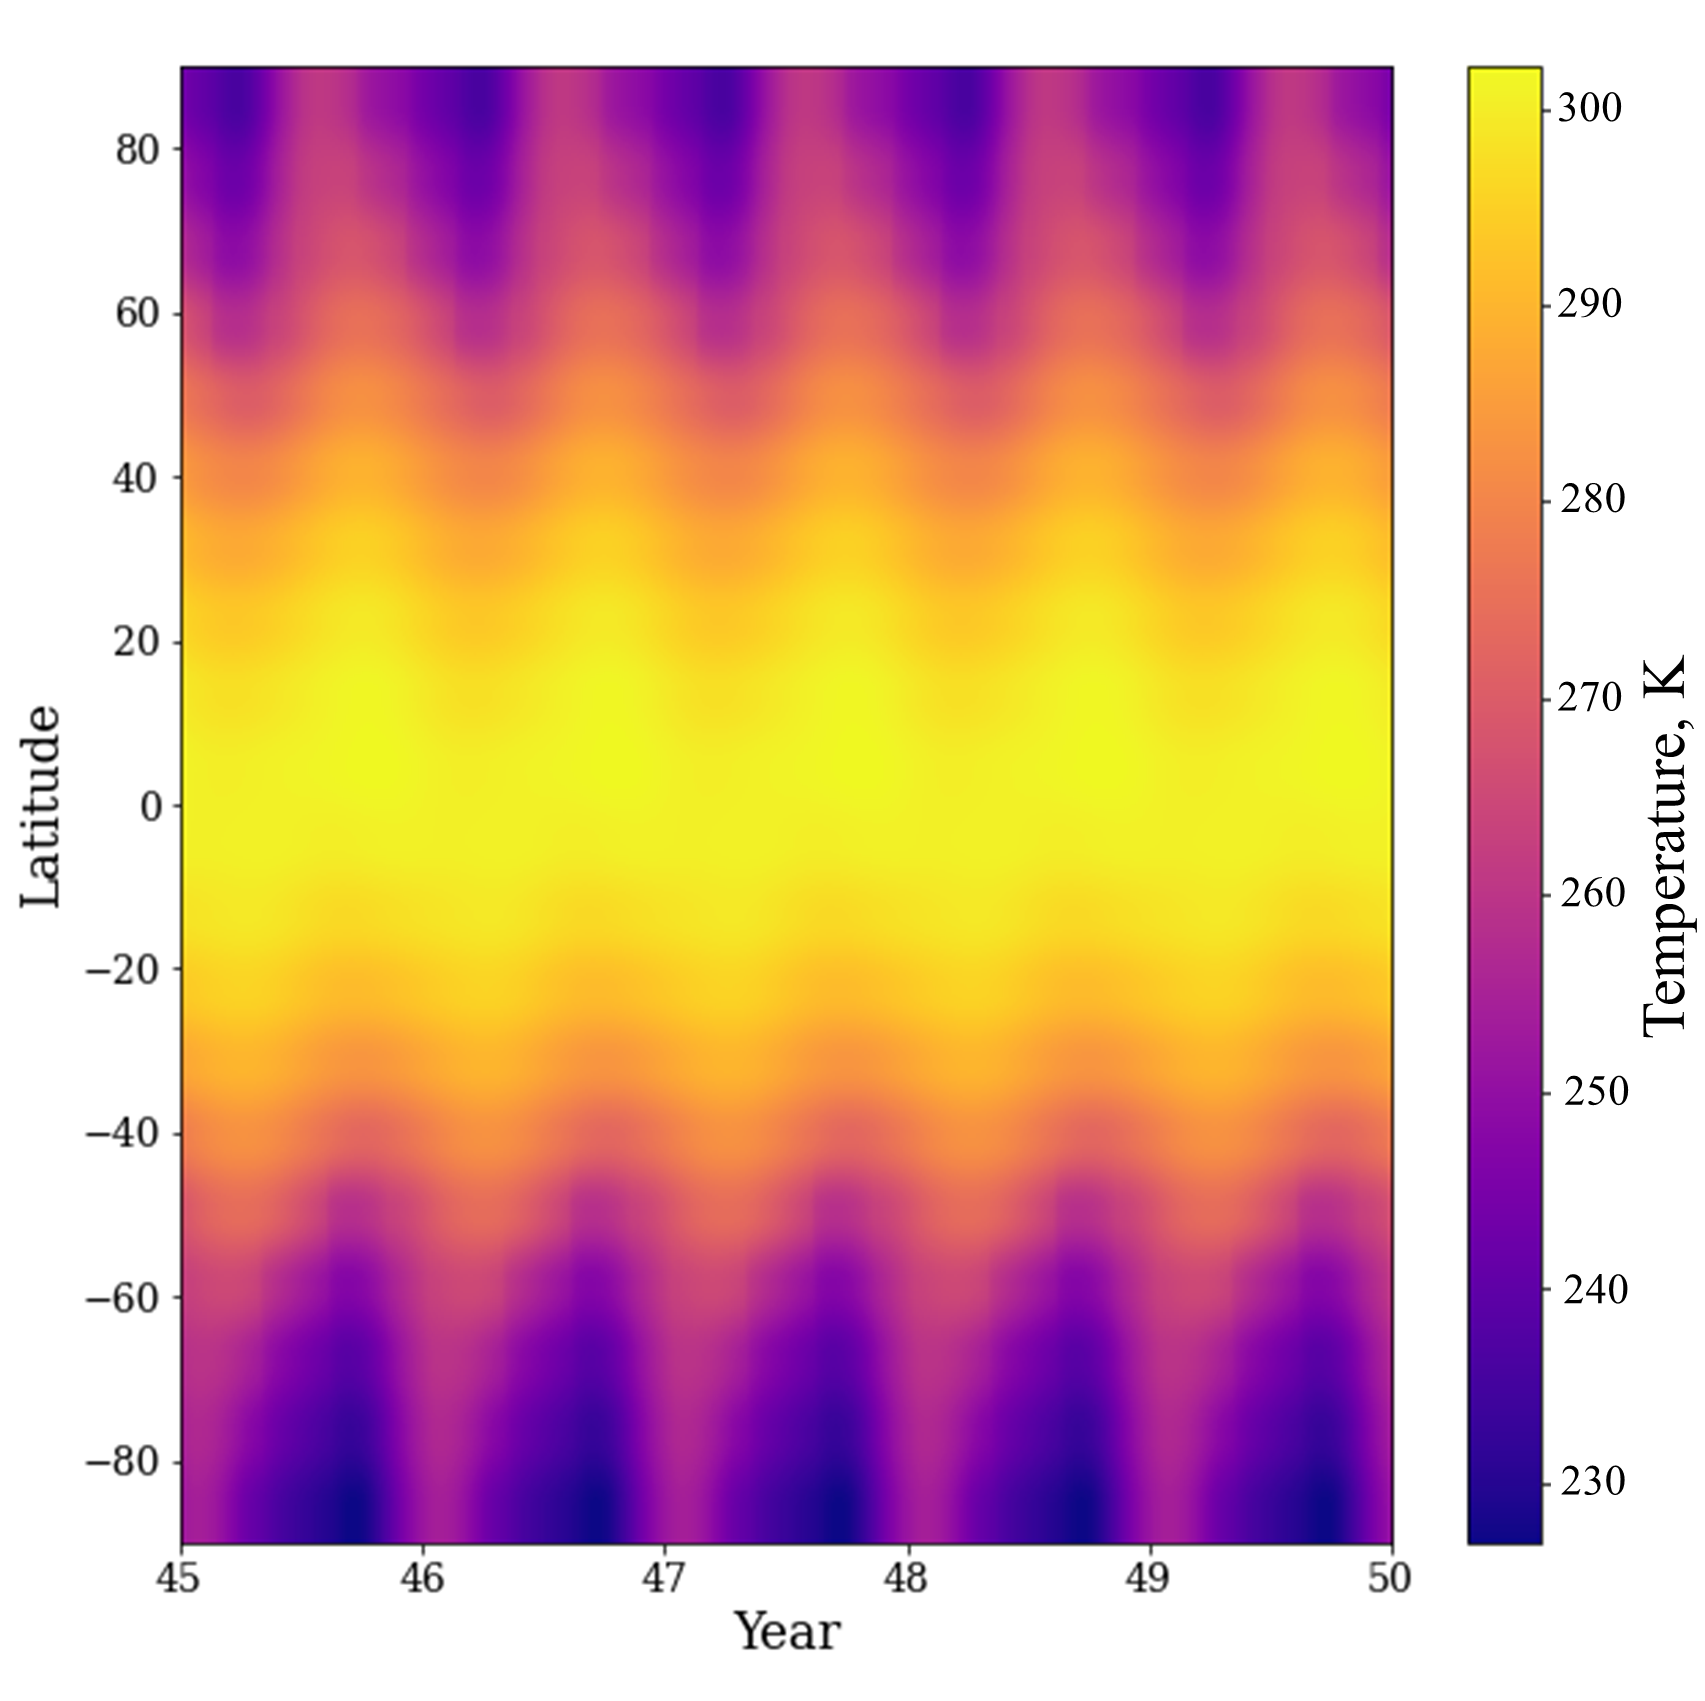
\includegraphics[width = 14cm]{Earth5yrsHeatmapNew.png}
\caption{Heatmap displaying 5 Earth years of the model solution (Kelvin). Heatmap taken once solution has converged.}
\label{fig:test}
\end{figure}

\begin{figure}[H]
%\centering
\begin{subfigure}{.5\textwidth}
  \centering
  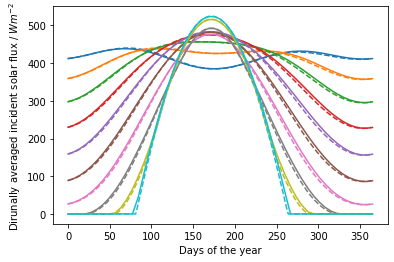
\includegraphics[width = 8cm]{EarthNorthFlux.png}
  \caption{Northern hemisphere}
  \label{fig:sub1}
\end{subfigure}%
\begin{subfigure}{.5\textwidth}
  \centering
  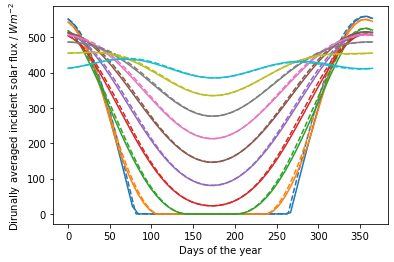
\includegraphics[width=8cm]{EarthSouthFlux.png}
  \caption{Southern hemisphere}
  \label{fig:sub2}
\end{subfigure}
\raggedright
\caption{Model data (dashed lines) plotted against calculated data (solid line) tabulated in \cite{K23} for Earths a) Northern, and b) Southern hemispheres. Flux shown at every 10$\degree$ of latitude. The dark blue line fluctuating about 400 Wm$^{-2}$ represents flux received at the equator.}
\label{fig:test}
\end{figure}

The model solution under Earth parameters is compared to an empirical model formulated from observational data \cite{NC79},

\begin{equation}
T(x) = 302.3 - 45.3 \sin^{2}\lambda,
\end{equation}

where $x$ $\equiv \sin\lambda$ is the sine of latitude and $T$ is temperature. This fit does not account for asymmetric seasonal variations induced by the inclusion of Earths obliquity, regardless, it describes the planets annual mean temperature per latitude well enough to assess the models' validity. A ten-year running annual mean is taken after every year of the models evolution past year 9. The mean relative difference across all latitudes is taken. The Earth model settles to a less than 1\% difference to the empirical model. Convergence is assessed by comparison to the above fit (Eq. 12) every year, and also comparison to the models own temperatures at the same point in orbit each year. The convergence tests are found in Fig. 3.

\section{Application to Present-Day Mars}
\subsection{Model Adaptations}

The model is adapted to reproduce present-day Mars by changing the obvious parameters: obliquity, semimajor axis, longitude of perihelion, eccentricity, and year length. These values change the amount of solar insolation, \textit{S}, the planet (and each latitude) receives. Values for land, ocean, and ice heat capacities are taken to be the same as for Earth, but the temperature value at which the heat capacity changes is altered to reflect the freezing point of carbon dioxide, rather than water. The land-ocean distribution disappears given that Mars has no land-ocean distribution. The outgoing radiation term is swapped out for a function which is dependent on the carbon dioxide pressure. 

\

\begin{figure}[H]
%\centering
\centering
\includegraphics[width = 16cm]{mars_flowchart.png}
\caption{Flowchart describing how the model runs to replicate Mars' climate. Orange tinted boxes highlight processes that happen at the same point as in the Earth model and serve the same purpose: input parameters are different, IR, albedo, and diffusive terms are adapted to reflect Mars. Additional data, such as ice cap thickness and pressure, are outputted. Green tinted boxes represent additions to the model.}
\label{fig:test}
\end{figure}

The albedo term is prescribed separately for the Northern and Southern hemispheres. In the North, it is largely similar to that of Earths, where instead of gently sloping between approximately 0.25 and 0.77 about the freezing point of water, it now does so about the freezing point of carbon dioxide. Albedo in the South is changed to ensure the permanence of the Southern ice cap - this energy balance model, and others, have difficulties maintaining the Southern ice cap while applying the Southern albedo measured via orbiters (this is discussed more in section [X]). The Martian dichotomy is further accounted for by calculating pressure separately in each hemisphere, owing to the severe altitude difference between the North and South.

\

Computational parameters, such as the number of latitude bands, are tuned to produce the most resolved image of Mars' climate while avoiding numerical instabilities associated with overresolution of the model. Timestep remains as $\Delta t$ = 1 day, given that solar irradiation is the mean over one day. The initial temperature is chosen again to be well above the freezing point (this time, of carbon dioxide) to avoid inescapable snowballing. The model is ran for t \textgreater 100 years to ensure its convergence.

\subsection{Incorporation of the $\mathrm{CO_2}$ Cycle for Mars}
%denser early atmosphere section of climate of early mars could be helpful

It is assumed that the amount of $\mathrm{CO_2}$ adsorbed and released from the regolith annually is negligible, so that the total conserved amount of $\mathrm{CO_2}$ on Mars is always split between ice on the ground and gaseous $\mathrm{CO_2}$ in the atmosphere. In the model, sublimation and condensation of $\mathrm{CO_2}$ happens instantaneously as the temperature drops below freezing point or as temperature rises above it, in a band where there is $\mathrm{CO_2}$ frost present. It is  also assumed that the entire atmosphere is composed of $\mathrm{CO_2}$ (reasonable given that it is in reality 95.32\% $\mathrm{CO_2}$ \cite{JN82}). To include the effects of $\mathrm{CO_2}$ condensation and sublimation on temperature, a latent heat term is required to alter Eq. 9.,  %need something about how much (hopefully negligible) is stored/released from regolith annually 

\begin{equation}
C \frac{\partial T}{\partial t} = S(1-A) + \frac{\partial}{\partial x} [D(1-x^{2})\frac{\partial T}{\partial x}] - I + \frac{\partial M}{\partial t},
\end{equation}

where $\frac{\partial M}{\partial t}$ is the mass of $\mathrm{CO_2}$ which condenses or sublimes per unit time. With the addition of the latent heat term, the differential equation behaves differently depending on the temperature at each band and the presence (or absence) of $\mathrm{CO_2}$ frost on the ground at that latitude. While both temperatures remain above the freezing point of $\mathrm{CO_2}$, and there is no $\mathrm{CO_2}$ frost, the model behaves as described earlier and finds $\frac{\partial T}{\partial t}$. The freezing point itself is a function of pressure, 

\begin{equation}
T_{c} = \frac{3148.42}{26.388 - \ln{p}},
\end{equation}
\

\begin{figure}[H]
%\centering
\centering
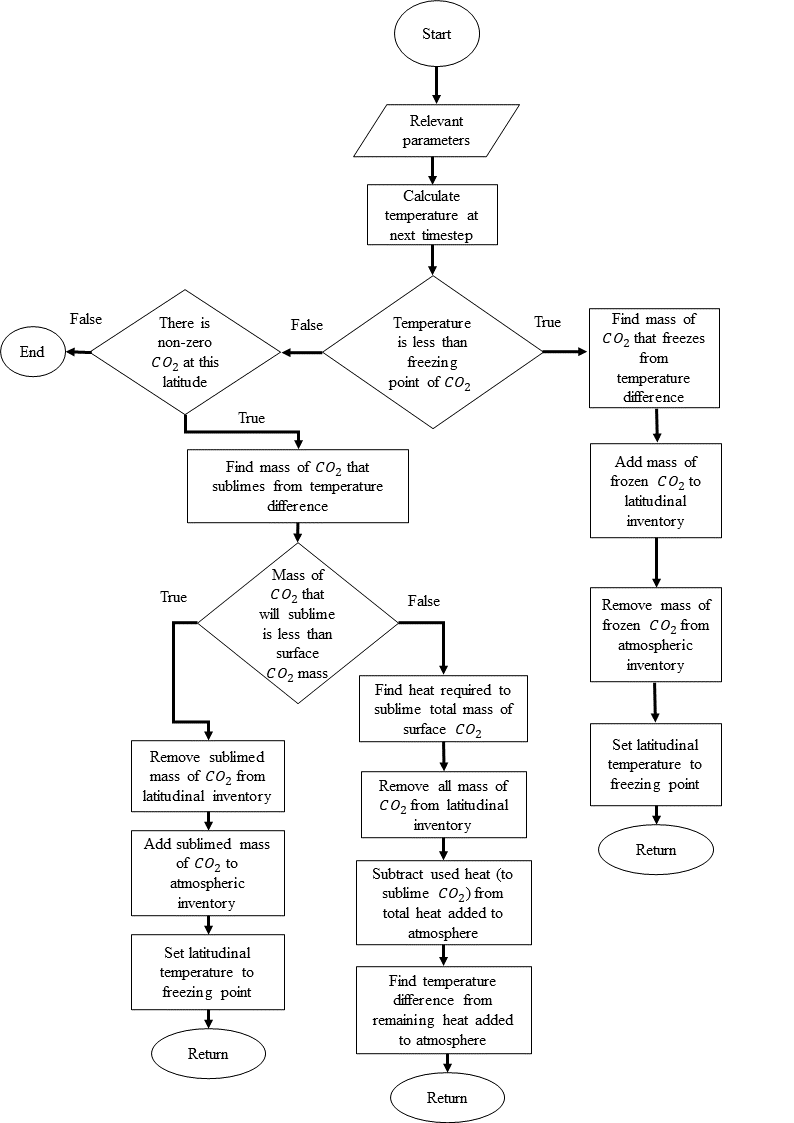
\includegraphics[width = 15cm]{flowchart2.png}
\caption{Flowchart describing implementation of the carbon dioxide algorithm. Parallelograms represent inputs to the function, rectangles represent mathematical processes, and diamonds represent decisions. The relevant parameters mentioned in the input box include the latitude band, the most recent temperature at that band, condensed surface $\mathrm{CO_2}$ at that band, and the pressure in the relevant hemisphere. This decision-making process is repeated for every latitude band at each timestep - the above represents just one latitude at one timestep.}
\label{fig:test}
\end{figure}
\

where $p$ is measured in $\mathrm{kg m^{-2}}$ \cite{H54}. However, in the presence of $\mathrm{CO_2}$ frost, the $\frac{\partial T}{\partial t}$ is set to zero and the change in $\mathrm{CO_2}$ frost mass is calculated, since the presence of  $\mathrm{CO_2}$ frost effectively fixes the temperature at that point to the freezing point of $\mathrm{CO_2}$. Temperatures below the freezing point would result in the condensation of $\mathrm{CO_2}$, which releases latent heat and warms the local atmosphere. Conversely, energy added to the system sublimes frozen $\mathrm{CO_2}$, and heats the atmosphere once the surface is ice-free. The algorithm implemented to mimic the behaviour of the climate according to the presence of $\mathrm{CO_2}$ is further described by Fig.[X]. This balance results in an almost constant (pressure-dependent) temperature at the Southern pole, which retains a permanent frost cap year-round (ref?).  If all of the $\mathrm{CO_2}$ were to condense, thus allowing temperature to drop, the atmosphere would have collapsed in which case the model would not apply (the solar flux received by Mars would not allow the temperature to drop this low regardless).
\

The atmosphere-ice $\mathrm{CO_2}$ split is determined by conservation of mass, 
\begin{equation}
M_{total} = M_{atmosphere} + M_{ice},
\end{equation}
where the mass of condensed $\mathrm{CO_2}$ is determined by the areal extent and depth of the polar ice caps. In turn, mass of $\mathrm{CO_2}$ in the atmosphere is determined by assuming a conserved total $\mathrm{CO_2}$ mass $M_{total}$. Gaseous $\mathrm{CO_2}$ contributes to the atmospheric pressure, which affects the diffusion coefficient $D$ as described in Eq. 11. Additionally, pressure is taken as a global variable, rather than one which is latitudinally dependent, so pressure tides are not observed. Once global pressure is updated, pressure is estimated in each hemisphere by splitting them in a ratio according to the Martian altitude dichotomy. 

\

The Martian dichotomy is accounted for by calculating pressure separately in each hemisphere, owing to the severe altitude difference between the North and South. Assuming a thin, isothermal, ideal gas atmosphere, pressure drops exponentially with altitude,

\begin{equation}
P \propto e^{-h/H},
\end{equation}

from its initial surface value, $P_{0}$. It is dependent on scale height, $H$, the distance over which pressure drops to 1/e of its original value. Scale height is a function of surface temperature $T$, gravitational attraction $g$, and the composition of the atmosphere,

\begin{equation}
H = \frac{kT}{\mu m_{h} g}.
\end{equation}

Taking g = 3.72ms$^{-2}$, $\mu$ = 44.0 (assuming a pure $\mathrm{CO_2}$ atmosphere), and an average surface emission temperature of 218K \cite{M01}, scale height $H$ is approximately 11km. This results in the atmospheric pressure in the Southern hemisphere being approximately 76\% of that in the North, taking  $\Delta$h = 3km, given that the two hemispheres differ by 2 to 4km in altitude \cite{S04}. The pressure at each latitude band is found by assessing whether it is Northern or Southern, then splitting the global atmospheric pressure total such that the value in the South is 83\% of that in the North. Differing pressures in each hemisphere are used to calculate the hemisphere-specific freezing point for $\mathrm{CO_2}$. The Southern hemisphere then, which reaches higher altitudes on average than the Northern hemisphere, feels smaller pressures than the North. While pressure in each hemisphere is not plotted, this will affect temperature and frost depth.

\

Rather than reusing the outgoing radiation prescriptions proposed in section \textbf{II. A.}, the partial pressure of $\mathrm{CO_2}$ should be considered in a parametrisation of outgoing IR in order to account for the greenhouse effect - which will have little effect on present-day Mars, but is integral to the study of Noachian-era Mars. Nakamura and Tajika achieved this with a linear function of the same form as model 3 in table I,

\begin{equation}
\begin{aligned}
I(T>T_{0}) = A_{1} + B_{1}T
\\
I(T \le T_{0}) = A_{2} + B_{2}T
\end{aligned}
\end{equation}

where coefficients A and B were simple functions of powers of $\rho$, the log of surface pressure of $\mathrm{CO_2}$ above and below $T_{0}$ \cite{NT01}. The fitting parameters, which are determined by Nakamura and Tajika from earlier radiative-convective calculations, are found in table [X]. It should be noted that this parametrisation does not account for either $\mathrm{CO_2}$ or $\mathrm{H_2 O}$ cloud cover

\begin{table}
\begin{tabular}{ccccc} \toprule
    n & $a_{n} (A_{1})$ & $a_{n} (A_{2})$ & $b_{n} (B_{1})$ & $b_{n} (B_{2})$ \\ \midrule
    1  & 0.6449 & 0.1068 & -0.003256 & -0.00094 \\
    2  & 13.28 & 2.198 & -0.06758 & -0.0195 \\
    3  & 99.54  & 16.48 & -0.5069 & -0.1464 \\
    4 & 329.9 & 54.64 & -1.68 & -0.485      \\
    5 & -372.7 & -61.72 & 1.898 & 0.5479
\\

\bottomrule
\end{tabular}
\caption{Fitting parameters for the outgoing infrared radiation function (Eq. [X]). $T_{0}$ = 230.1K. }.
\end{table}

The diffusion coefficient described in Eq. \ref{diffusionequation} is now variable, dependent on the pressure at each latitude band (which is in turn dependent on the altitude dichotomy pressure split). It is calculated for each latitude band daily.

\subsection{Model solutions for Mars}
Mars' model climate is compared to an analytical fit \cite{KH18} which is based on results from the NASA Ames GCM for a 7 millibar atmosphere, 

\begin{equation}
T(x) = \frac{q_{0}}{4 \sqrt{1 - e^{2}}} \frac{S_{a_{0}}}{B} - \frac{A}{B} + \frac{q_{0}}{4 \sqrt{1 - e^{2}}} (\frac{S_{a_{2}}p_{2}(x)}{6D+B} + \frac{S_{a_{4}}p_{4}(x)}{20D+B}),
\end{equation}

where $q_{0}$ is the solar constant at Mars, $e$ is eccentricity, $D$ is diffusivity, and $x$ $\equiv \sin\lambda$ is the sine of the latitude. $S_{a_{n}}$ are the net solar insolation parameters, which are dependent on obliquity, direct insolation, and annually averaged co-albedo coefficients. The Legendre polynomials are represented by $p_{n}$. $A$ and $B$, found in table \ref{table:GCMparams}, are outgoing longwave radiation parameters which describe the linear relation between temperature and outgoing radiation.

\begin{figure}[h]
%\centering
\centering
\includegraphics[width = 16cm]{mars_flux_new.png}
\caption{Solar flux received by Mars at 32 latitude points over one Martian year. The larger curve corresponds to the Southern summer hemisphere, and the smaller one to the Northern summer.}
\label{fig:marsflux}
\end{figure}

\

\begin{table}
\begin{tabular}{cccc} \toprule
    Pressure (millibar) & $D$ & $A$ & $B$ \\ \midrule
    7  & 0.02 & -212 & 1.54 \\
    3500 & 1.28 & 13 & 0.23 \\
\bottomrule
\end{tabular}
\caption{Outgoing longwave radiation fitting parameters from NASA Ames GCM. The 3500 millibar case is listed here for use in the investigation of ancient Mars.}
\label{table:GCMparams}
\end{table}

\

\begin{figure}[h]
%\centering
\centering
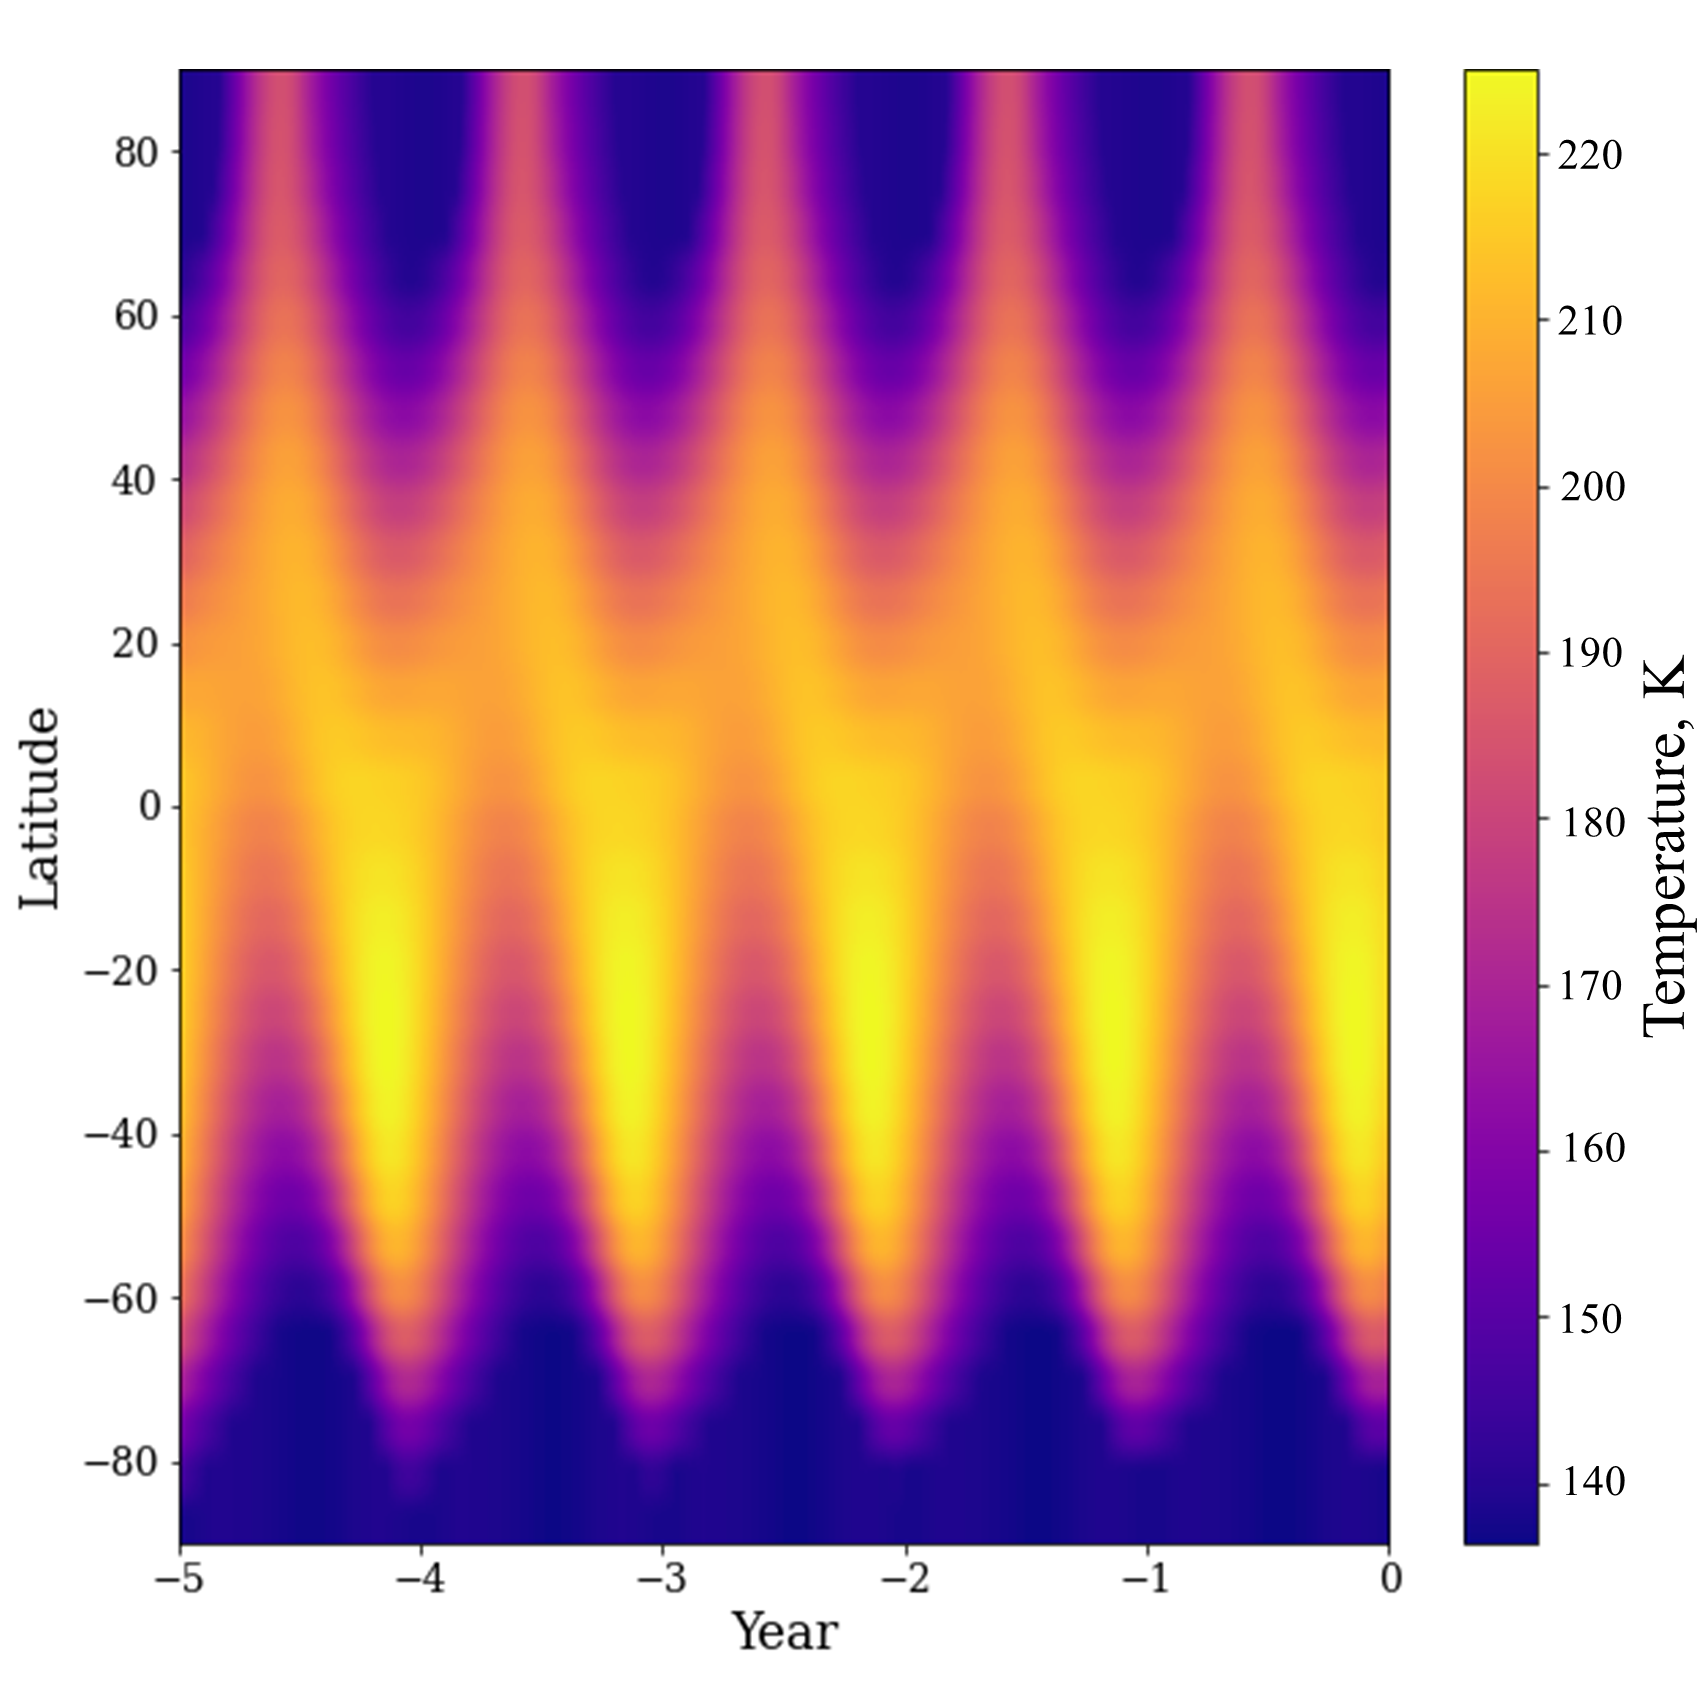
\includegraphics[width = 14cm]{Mars5yrsHeatmapNew.png}
\caption{Heatmap displaying 5 Martian years of present-day Mars' climate (Kelvin). Heatmap taken once solution has converged.}
\label{fig:modernmarsheatmap}
\end{figure}

The diurnally averaged solar insolation for various latitudes is found in Fig. \ref{fig:marsflux}. It is expected that solar insolation will peak at perihelion, observed around day 500 in the graph, at a value approximately $\frac{1}{1.38^{2}}$ that of Earths peak insolation given that Mars' closest pass by the Sun is at 1.38AU. Similarly, solar insolation should have a maximum of $\frac{1}{1.67^{2}}$ that of Earths maximum at Mars' aphelion, which occurs at 1.67AU. Both of these are observed in Fig. /ref{fig:marsflux}, with the smaller and larger peak having values of 184 Wm$^{-2}$ and 267 Wm$^{-2}$ respectively. 

\

The solution for present-day Mars, shown in Fig. \ref{fig:modernmarsheatmap}, displays characteristic features observed on Mars today. The Southern hemisphere shows extreme seasonal changes in comparison to the North, as a result of Mars' perihelion occurring during the Southern summer and producing large temperature increases. The Southern pole also has a permanent $\mathrm{CO_2}$ ice cap, in contrast with the Norths temporary $\mathrm{CO_2}$ ice cap, which sublimes completely during the summer. Mars' climate overall is also much more extreme in comparison to Earths, owing to its much sparser atmosphere which does not favour cross-latitudinal heat diffusion. The pressure cycle is investigated, along with ice cap depth and extent, as a validation exercise for the model. Mean pressure is found to be 73.8 $kgm^{-2}$ (or 7.2 millibar), in comparison with x $kgm^{-2}$ (or x millibar) found recently [here].

\

In some ways, the Mars climate model is a more valid solution than the Earth model. The assumption of evenly distributed ocean and land in the parametrisation of heat capacity is, of course, entirely justified on Mars given that it is 100\% land. Present-day Mars additionally has few extreme weather events in comparison to Earth, so disregarding the effects of $\mathrm{H_2 O}$ and $\mathrm{CO_2}$ clouds is valid.

\ 

Viking missions show a variation of around 25\% in surface pressure over the course of a year, between lows of 69 millibar to highs of 100 millibar - this is dependent on a variety of variables such as latitude, altitude, and the presence of dust storms. Viking landers 1 and 2 find the same shape of pressure cycle, with peaks and troughs occurring at the same time in the Martian year, but at different amplitudes due to the latitude of their landing sites. Viking Lander 1 is considered more representative of the Martian atmosphere, owing to its placement at 22 $\degree$ North in comparison to Viking Lander 2's placement at 48 $\degree$ North, and it measures a lower magnitude of pressure variation than VL2. Martian pressure cycles follow a characteristic shape including two annual peaks, and two troughs, of variable sizes as a result of the $\mathrm{CO_2}$ sublimation and condensation cycle. The deepest pressure trough occurs around Ls = 150 $\degree$, during Southern winter. It is the most severe pressure drop of the year for the same reason that the Southern hemisphere has such severe seasons: the eccentricity of Mars' orbit creates a much longer winter in the South than in the North, and as a result more $\mathrm{CO_2}$ will condense at the poles and be removed from the atmosphere. The smaller minimum occurs around Ls = 0 as a result of the Northern winter, which is shorter, warmer, and therefore removes less $\mathrm{CO_2}$ from the atmospheric inventory.

\

\begin{figure}[H]
%\centering
\centering
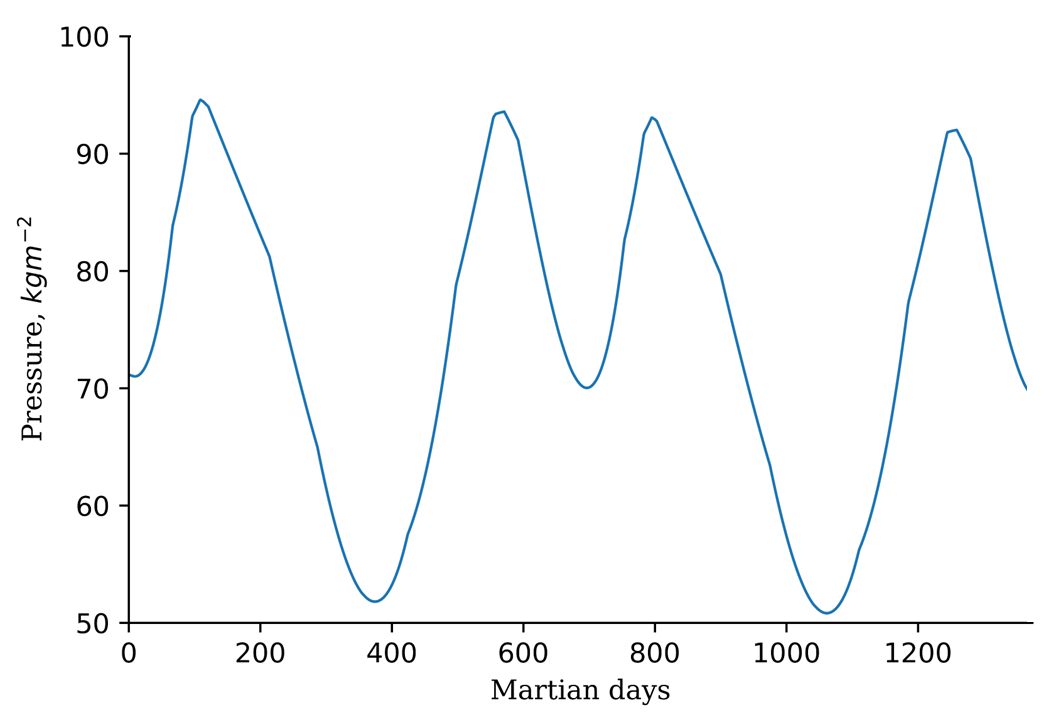
\includegraphics[width = 14cm]{mars_pressure2.png}
\caption{Pressure on Mars throughout two Martian years. Two cycles are shown for clarity on the shape of the pressure cycle.}
\label{fig:test}
\end{figure}

\

The same trend of deep minima separated by smaller minima is observed in the model recreation of the pressure cycle. A deep trough around 51 millibar occurs during Southern winter into spring as expected, while the Southern ice cap is at its largest extent. A smaller trough of 71 millibar occurs at the Northern spring equinox (or Southern autumn equinox), Ls = 0 $\degree$, corresponding to the sublimation of the temporary Northern $\mathrm{CO_2}$ ice cap. Similarly, the two peaks should differ in magnitude: the Southern summer perihelion peak should be larger than the Northern spring peak, given that the smaller Northern winter results in a smaller deposit of $\mathrm{CO_2}$. However in the model recreation, these peaks are of similar magnitude (93 millibar and 92 millibar for the large and small peak, respectively).

\

These maxima and minima are similar in magnitude to the highs and lows measured by the Viking Landers, but slightly lower (around 10 millibar) than expected. The pressure cycle produced by the model is dependent on the total $\mathrm{CO_2}$ inventory specified at the beginning of the model. Increasing the amount of available $\mathrm{CO_2}$ to begin with does shift the whole cycle upwards to within the expected range (60-100 millibar), however it also increases the mean surface pressure to 90 millibar, which is an unreasonable estimate. It is possible that this shift is the correct shift to make, however the slightly altered shape of the model pressure cycle shifts the mean higher than it should be. Given that the Northern spring peak is more pronounced than it should be in comparison to the perihelion peak, the mean value of pressure will be slightly larger than a more accurately shaped cycle, with a smaller spring peak, would provide. Optimising the mean surface pressure was prioritised over correcting the range in order to more accurately estimate the cap-atmosphere $\mathrm{CO_2}$ inventory.

\

In initialising the model, all $\mathrm{CO_2}$ begins in the atmospheric inventory. It could be argued that changing the initial distribution to be representative of present-day Mars at the same point in orbit as the model is initialised could affect the final solution $\mathrm{CO_2}$ distribution and therefore, the climate. However, given that the albedo parametrisation is independent of frost depth and only dependent on temperature, it is unlikely that specifying an initial state would affect the final stable climate solution.

\

It has been found that, while the Martian regolith could store a substantial share of Mars' $\mathrm{CO_2}$ inventory, seasonal exchange between the atmosphere and ice caps is a far more significant driver of yearly climate change than regolith-atmosphere exchange. Net atmosphere pressure variations as a result of neglected atmosphere-regolith exchange are estimated to be less than 0.14 millibar \cite{FBSJS82}, regardless of soil geometry and temperature, suggesting the neglect of regolith $\mathrm{CO_2}$ stores is justified. This pressure variation is negligible in comparison to the pressure variations displayed in our pressure cycle in Fig. [X] and in comparison to recent daily and seasonal cycles \cite{H24}. Additionally, while release of $\mathrm{CO_2}$ potentially from the regolith is an important mechanism for realising a denser climate in Noachian-era investigations, seasonal exchange remains insignificant on the short timescales the model is investigating (tens to hundreds of years). It is therefore justified to use a constant value of initial $\mathrm{CO_2}$ during present-day and ancient Mars, and disregard any marginal change in available $\mathrm{CO_2}$ that might occur over tens or hundreds of years.
Previous EBMs have also excluded the contribution of the regolith and reached the same conclusions as models including it \cite{NT01}.

\

The inclusion of a separate albedo parametrisation for the South pole was necessary in order to maintain the Southern ice cap: without it, the Southern cap sublimes completely during summer resulting in much larger pressure variations than observed on Mars. The parametrisation of albedo in the model also disregards the effect of $\mathrm{CO_2}$ on the reflective properties of the Martian surface. Albedo should in practice increase with increasing frost depth up to a maximum value, whereas here, it is taken solely as a function of temperature. The parametrisation in this work instead attempts to account for anomalous behaviour in the Southern polar region. Measured albedoes at the Southern cap do not reflect the energy balance deemed necessary, via modelling, for the Southern hemisphere to retain a permanent $\mathrm{CO_2}$ ice cap. In fact, when the albedo measured by the Viking Infrared Thermal Mapper is applied to a simple annual energy balance, the temperatures calculated suggest that the Southern hemisphere should not retain a permanent ice cap \cite{K79}. Other EBMs similarly have this problem, and apply different prescriptions of albedo to maintain the Southern ice cap \cite{FHT98} \cite{JN82}. The albedo used in this work is applied to the entire Southern hemisphere, and is tuned to reproduce as best as possible the "usual" albedo values expected at the mid-latitudes, and the abnormally high ones at the poles. This was done to ensure a smooth transition between ice-free and ice-covered states. While a more simple implementation, that is to set abnormally high constant albedoes at the Southern pole and apply the same Northern albedo function elsewhere in the South, produces similar results, it also produces temperatures discontinuities in the model as a result of the step-function-like albedo. It is possible that, during the winter, a significant fraction of $\mathrm{CO_2}$ condenses at mid-latitudes (releasing latent heat there) and is transported via suspension to the poles. This phenomenon would account for the low outgoing radiation measured in the South pole, however, it is expected that net transport of suspended $\mathrm{CO_2}$ would be towards mid-latitudes. The permanence of the Southern $\mathrm{CO_2}$ cap remains a mystery. The albedo at both poles is also, in reality, not nearly as symmetric as assumed by the model. While it is generally a much more valid assumption to take an invariant land distribution - owing to Mars' lack of oceans in comparison to Earth - the polar ice caps prove an exception to this. They are frequently described as having a "swiss cheese" appearance, with grooves within the caps which collect atmospheric dust. Albedo therefore varies depending on latitude and longitude. More importantly, the cap itself can become asymmetric depending on the time of year. This is not accounted for within the model, which provides latitudinally averaged results for temperature, and therefore its dependent variables (for example, cap thickness and albedo). 

\

Accounting for the altitude dichotomy by redistributing the atmospheric $\mathrm{CO_2}$ inventory results in a decrease of ice cap condensation and thus, less severe pressure dips. However, the net increase in atmospheric pressure is small - mean atmospheric pressure increases by only 1\% with the inclusion of the dichotomy, and condensation only drops by 6\% of the its previous value. Other EBMs have reported a 10\% reduction in $\mathrm{CO_2}$ condensation in the Southern pole \cite{JN82}. The altitude dichotomy could be accounted for dynamically instead - i.e., to find the scale height each day (either as a function of global mean temperature, or temperature per latitude), recalculate the pressure dichotomy this would create, and distribute pressure accordingly. 

\

Dust storms and their effects have not been included in the model. Such storms absorb and re-emit infrared radiation to produce an almost greenhouse-like effect, and also dramatically increase the mean atmospheric opacity of the planet (as discussed in section I) \cite{WR15}. The exclusion of dust storms likely cools the model, and could explain why the model doesn't reach the same amplitude of temperature extremes as observed by Viking landers, to highs in the 260-270K range \cite{K76}.

\section{Investigation of Ancient Mars}
\subsection{Exploring Orbital Parameters and the Faint Young Sun Paradox}

As discussed earlier, it is possible that the severe change in Mars' climate between the Noachian era and the present day was driven, at least partially, by cyclical variations in orbital parameters known as Milankovitch cycles. It is fundamental to understand the role each parameter plays in the control of the climate in order to assess the conditions under which Mars was most likely to host liquid water. The effects of varying obliquity and eccentricity were investigated under present-day conditions. These results are found in Figs. [X] and [X].
\\

It is important to note the unpredictable evolution of any parameter associated with Milankovitch cycles, and especially those pertaining to Mars. Milankovitch cycles are much more chaotic than simple sinusoidal variations, dependent on various resonances within the Solar system, and thus finding a true range of values for any particular time period in Martian history is impossible. Analytical approaches involving backward-integration through time produce wildly differing results past 100Myr ago, for initial conditions that vary only by the order of an arcsecond. Attempts to simplify these analytical approaches by discarding all but the two dominant terms still produces vastly different trajectories for almost indifferent initial conditions. It is for this reason that this work investigates such a seemingly wide range of obliquity and eccentricity possibilities. Mars' obliquity is estimated to have varied between 0 and 60 \degree by the aforementioned numerical/analytical methods, and its eccentricity between 0 and 0.14. These estimates inform the range of parameters investigated below.

\

Interestingly, Earth's obliquity is much more stable, varying only by $\pm$1$\degree$. It seems that its obliquity is stabilised by the presence of a large moon - Earth's spin precession is dominated by torques from the Moon, rather than the Sun. Its precession frequency is therefore much higher than the frequency of other orbital variations, and the space between these frequencies leads to fewer resonances and a less chaotic cycle. Mars' moons, Phobos and Deimos, are too small to create a stabilising effect.

\

\begin{figure}[H]
%\centering
\centering
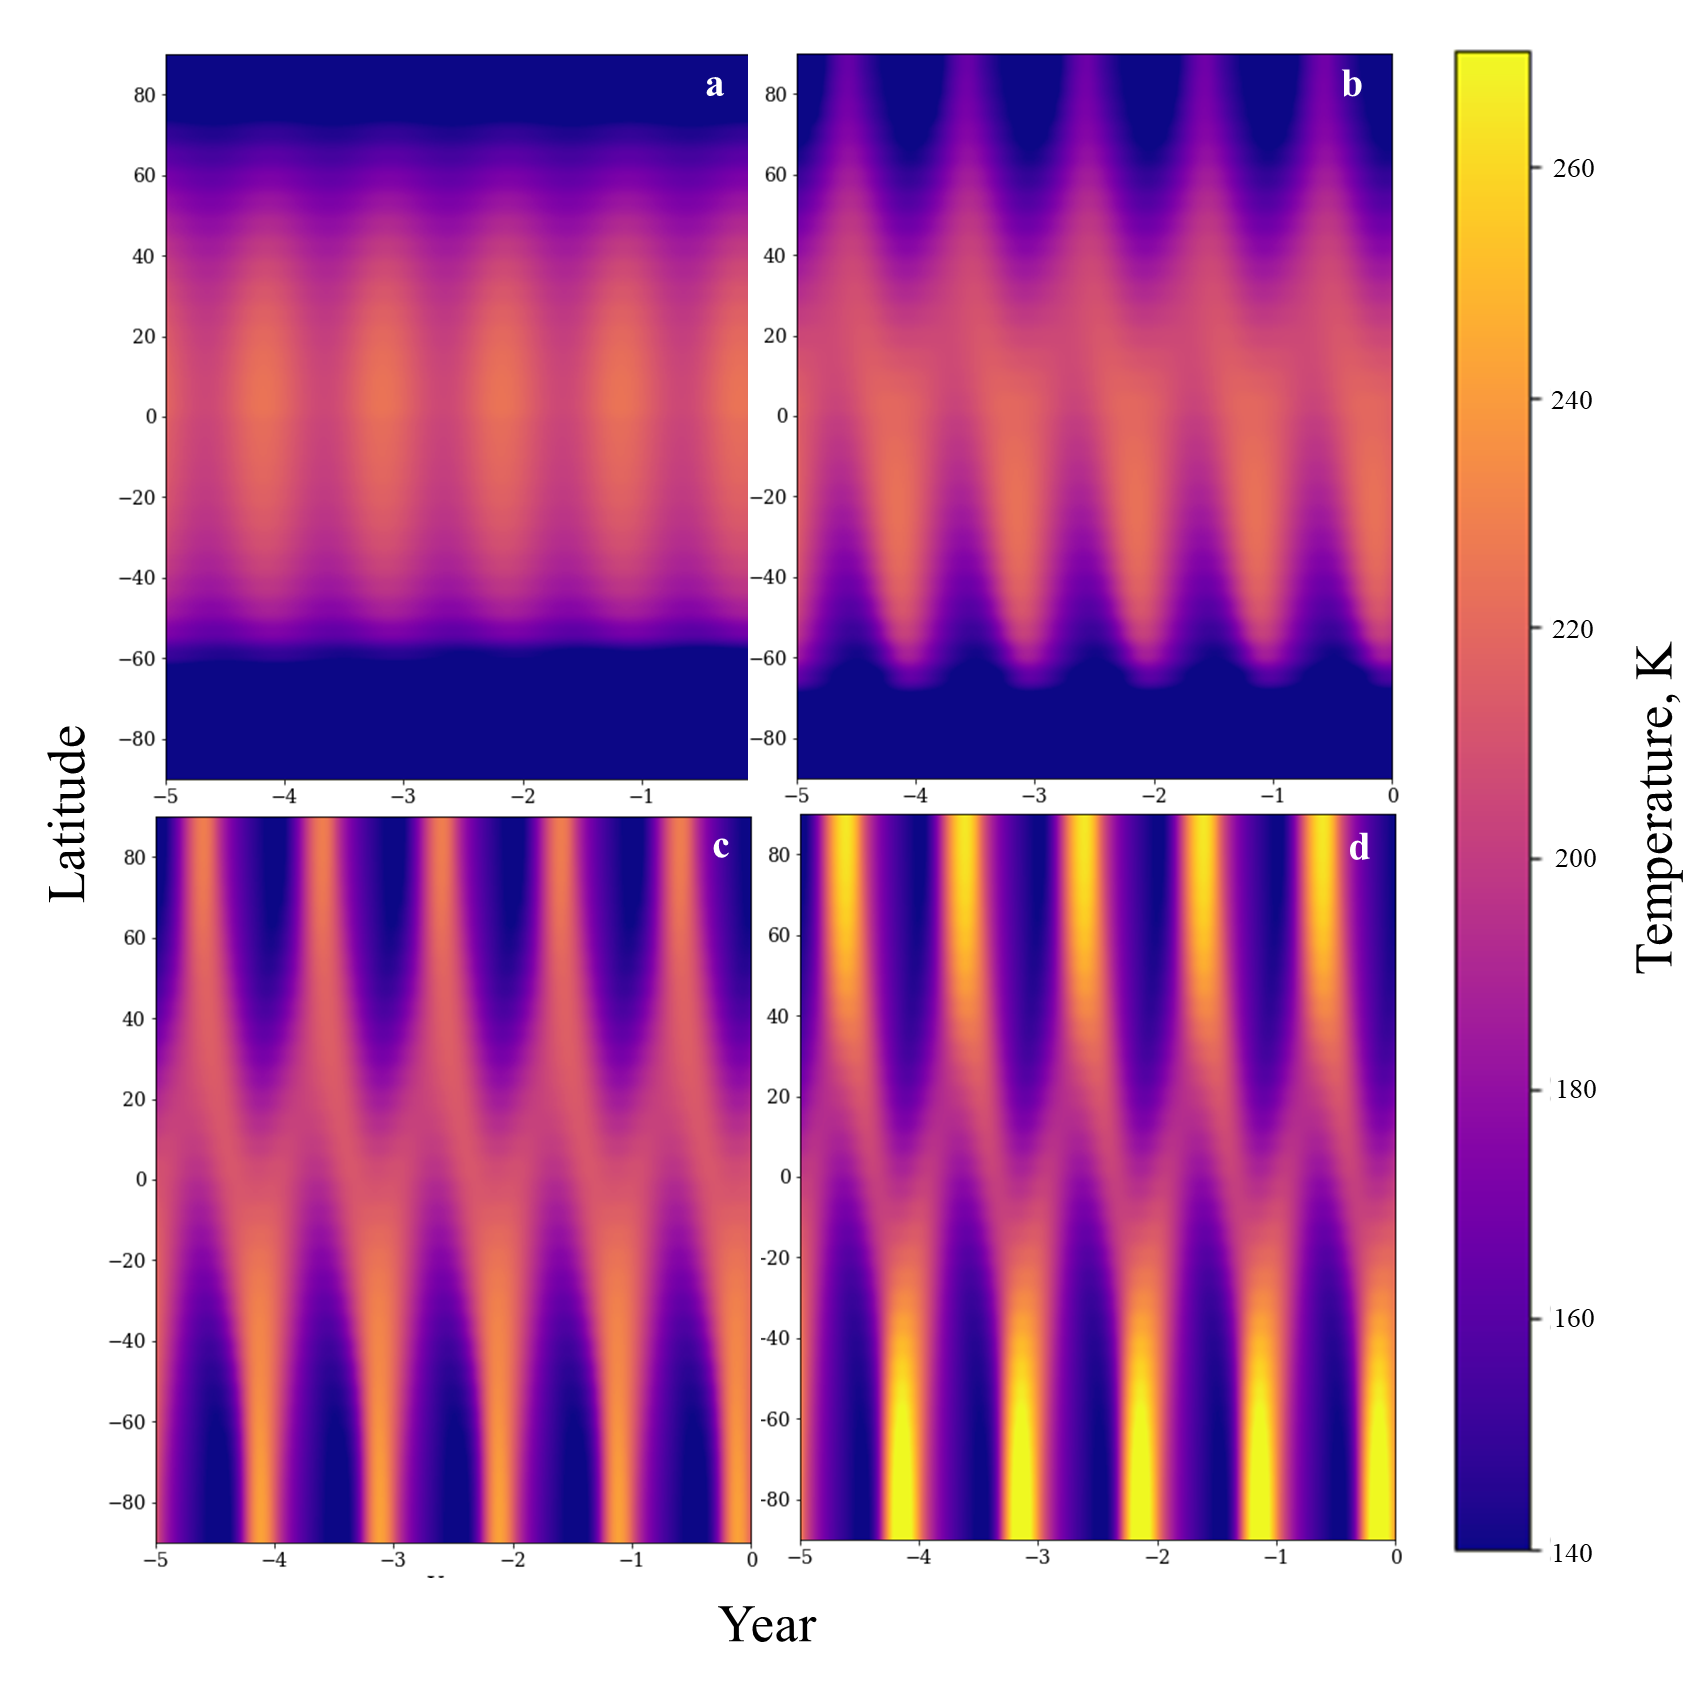
\includegraphics[width = 17cm]{obliquity_heatmaps_new.png}
\caption{The effects of obliquity on temperature (Kelvin), seasonal extremes, and ice cap stability. Obliquity increasing from 0$\degree$ to 60$\degree$ in 20$\degree$ increments from a) to d).}
\label{fig:test}
\end{figure}

Obliquity was varied between 0$\degree$ and 60$\degree$ in 10$\degree$ intervals. Heatmap b) in Fig. [X] largely resembles that of present-day Mars given it is only 5$\degree$ from its current axial tilt. With the increase, extreme seasons emerge, initially only obvious in the South. Southern extreme seasons are still a result of the Southern summer occurring close to perihelion, however the further warming of the North pole is a direct result of high obliquity states ($\phi$ \textgreater 53$\degree$). High obliquity states are defined as states in which the poles of a planet receive more annual mean solar radiation than the equator. This results in an inversion of the temperature gradient, which is seen clearly in heatmap d) ($\phi$ = 60$\degree$). Extreme obliquities plunge the poles into cold, extended winters when pointing away from the Sun, but result in much higher maximum temperatures during extended summer periods.
\\

\begin{figure}[H]
%\centering
\centering
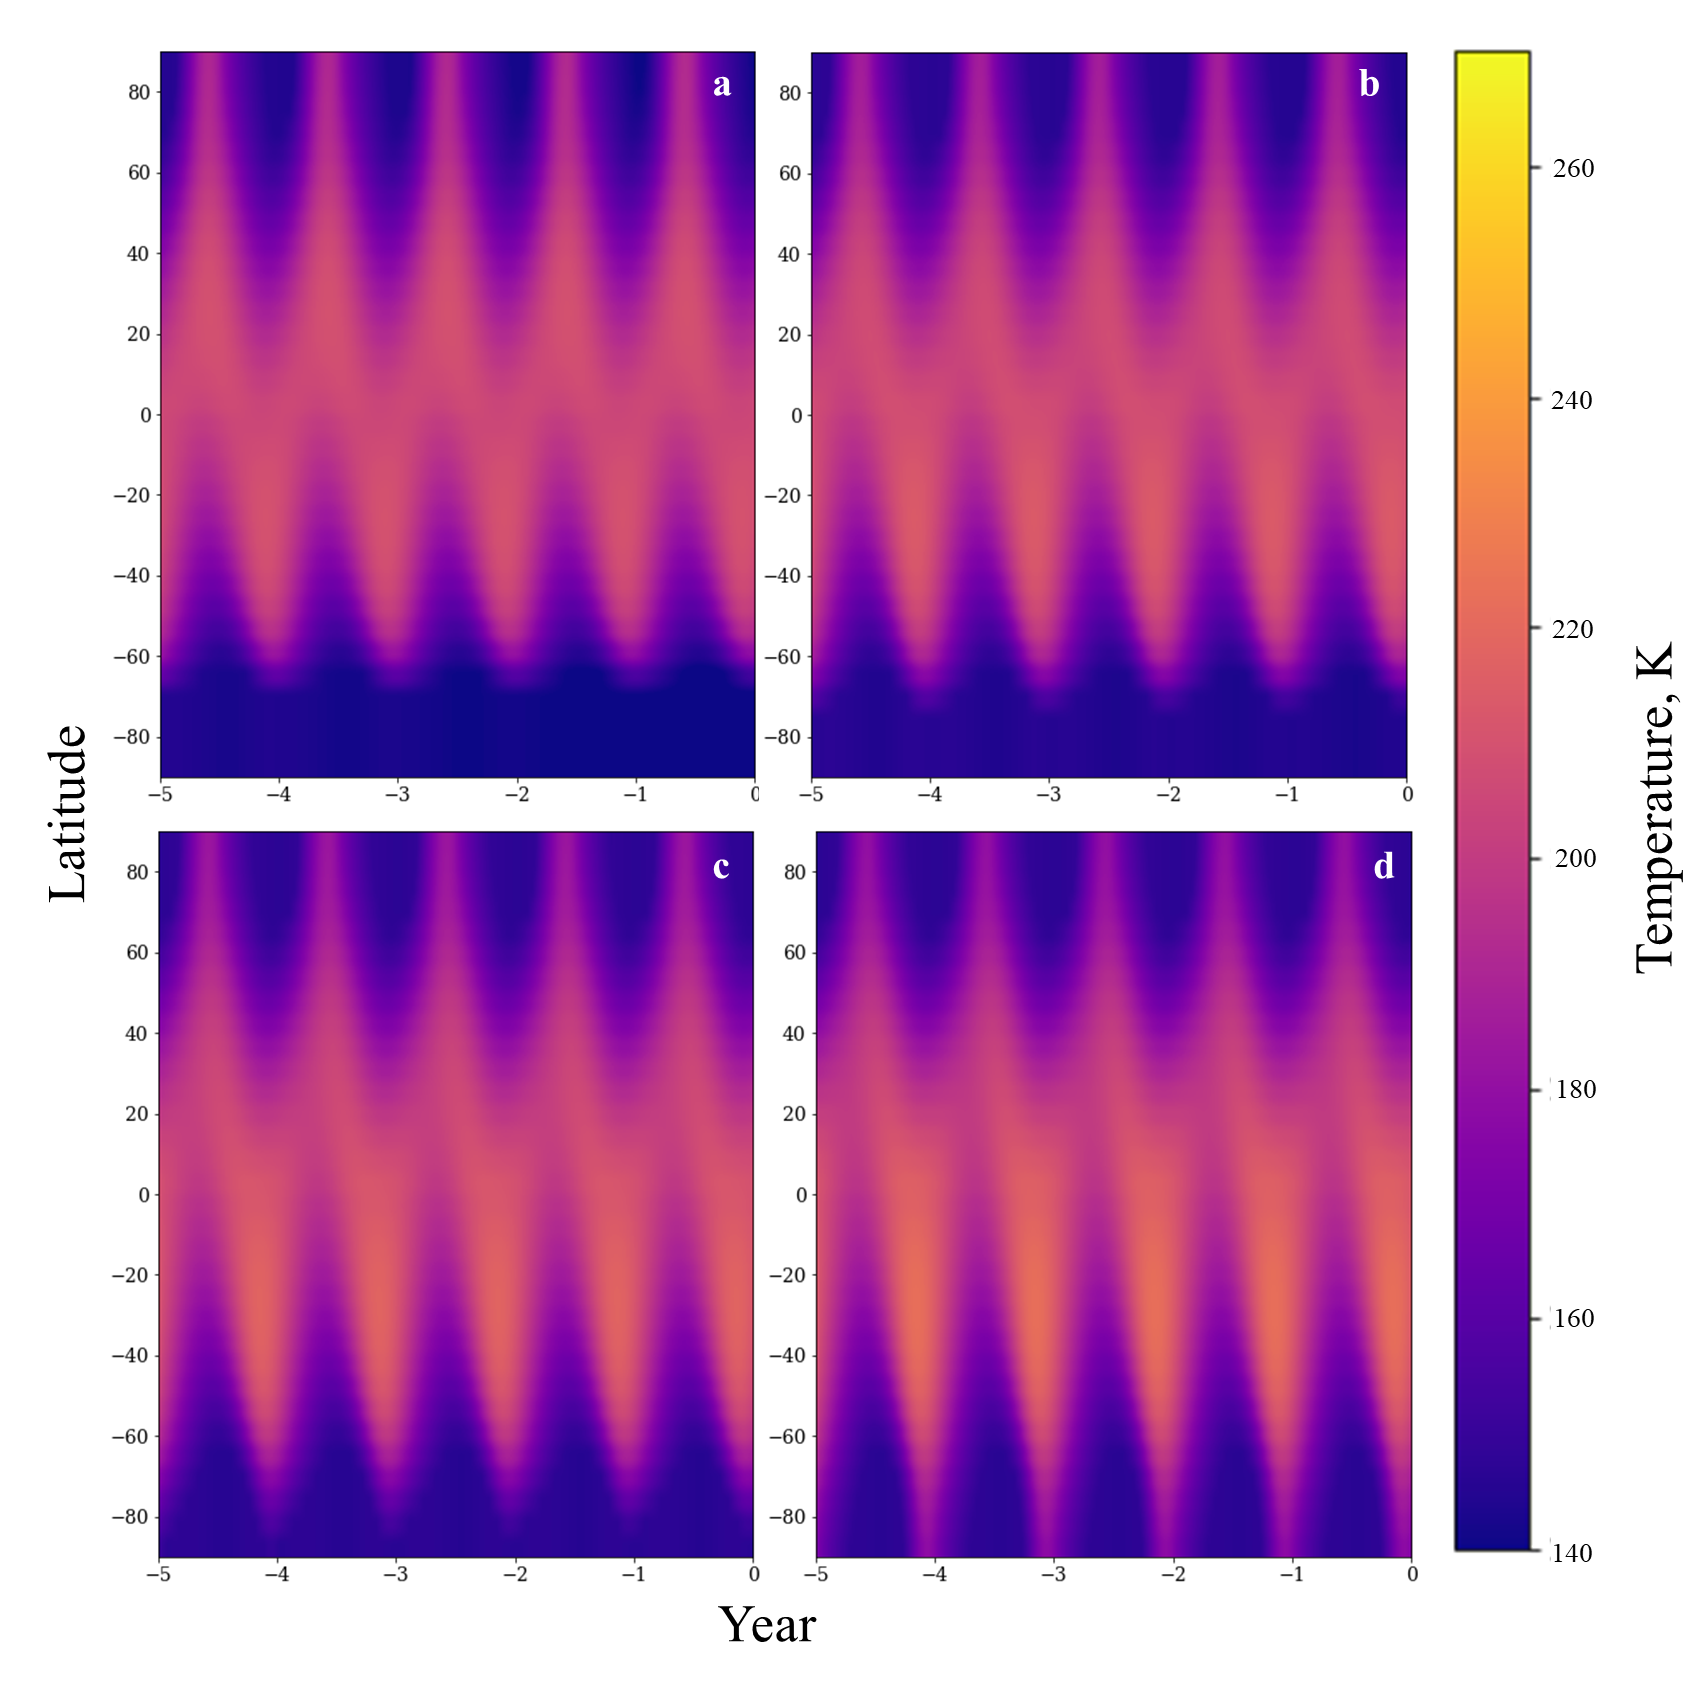
\includegraphics[width = 17cm]{eccentricity_heatmaps_new.png}
\caption{The effects of eccentricity on temperature (Kelvin), seasonal extremes, and ice cap stability. Eccentricity increasing from 0.02 to 0.14 in 0.02 increments from a) to d). The same colour bar is used as in Fig. [X] for ease of comparison to obliquity.}
\label{fig:test}
\end{figure}

Varying obliquity indirectly affects the pressure cycle, as a result of its effect on temperature. Higher temperatures at the poles result in temporary ice caps, releasing more $\mathrm{CO_2}$ into the atmosphere, and increasing the greenhouse effect which further warms the climate (a positive feedback mechanism). Higher temperatures also increase the freezing point of $\mathrm{CO_2}$, which acts to prevent further reduction of ice caps from higher temperatures (a negative feedback mechanism). The reduction of ice cap extent also reduces the mean albedo of the planet, allowing it to retain more heat and warm the climate. Additionally, the increase in heat transport coefficient (denoted in this work as D) allows for more efficient redistribution of heat across the planet, maintaining a mild climate at the mid-latitudes and equator. It is obvious then, from consideration of feedback mechanisms and investigation via modelling, that increasing the obliquity of Mars should warm its atmosphere.

\

Eccentricity was varied between 0 and 0.14 in steps of 0.02 to investigate its effects on the climate. The results are shown in Fig. [X]. Eccentricities larger than 0.10 result in the summer thawing of the Southern ice cap, and also a mild increase in temperatures most notable in the Southern mid-latitudes. High eccentricities also amplify the temperature disparity between the Northern and Southern hemispheres, as a result of the increased solar insolation at perihelion. Comparison to the variations of obliquity in Fig. [X] display how much more significant axial tilt is in influencing the climate in contrast to eccentricity.

\subsection{Model solutions for Ancient Mars}
The most extreme values (obliquity = 60$^{\circ}$, eccentricity = 0.14) are taken from the investigation into Martian orbital parameters in order to give Mars the best chance of reaching temperatures exceeding 273K. Pressure is increased incrementally until any part of the model reaches T \textgreater 273K. The following heatmap, Fig. \ref{fig:ancientmars} is under 3.5 bar of carbon dioxide (total, shared between the ice caps and atmosphere). Temperatures break freezing at the Southern pole, and partially at the mid-latitudes, during Southern summer. Temperatures are consistently above the freezing point of $\mathrm{CO_2}$ resulting in the elimination of the ice caps and pressure cycle. Consequently, the atmosphere accounts for the whole $\mathrm{CO_2}$ inventory.

\begin{figure}[h]
%\centering
\centering
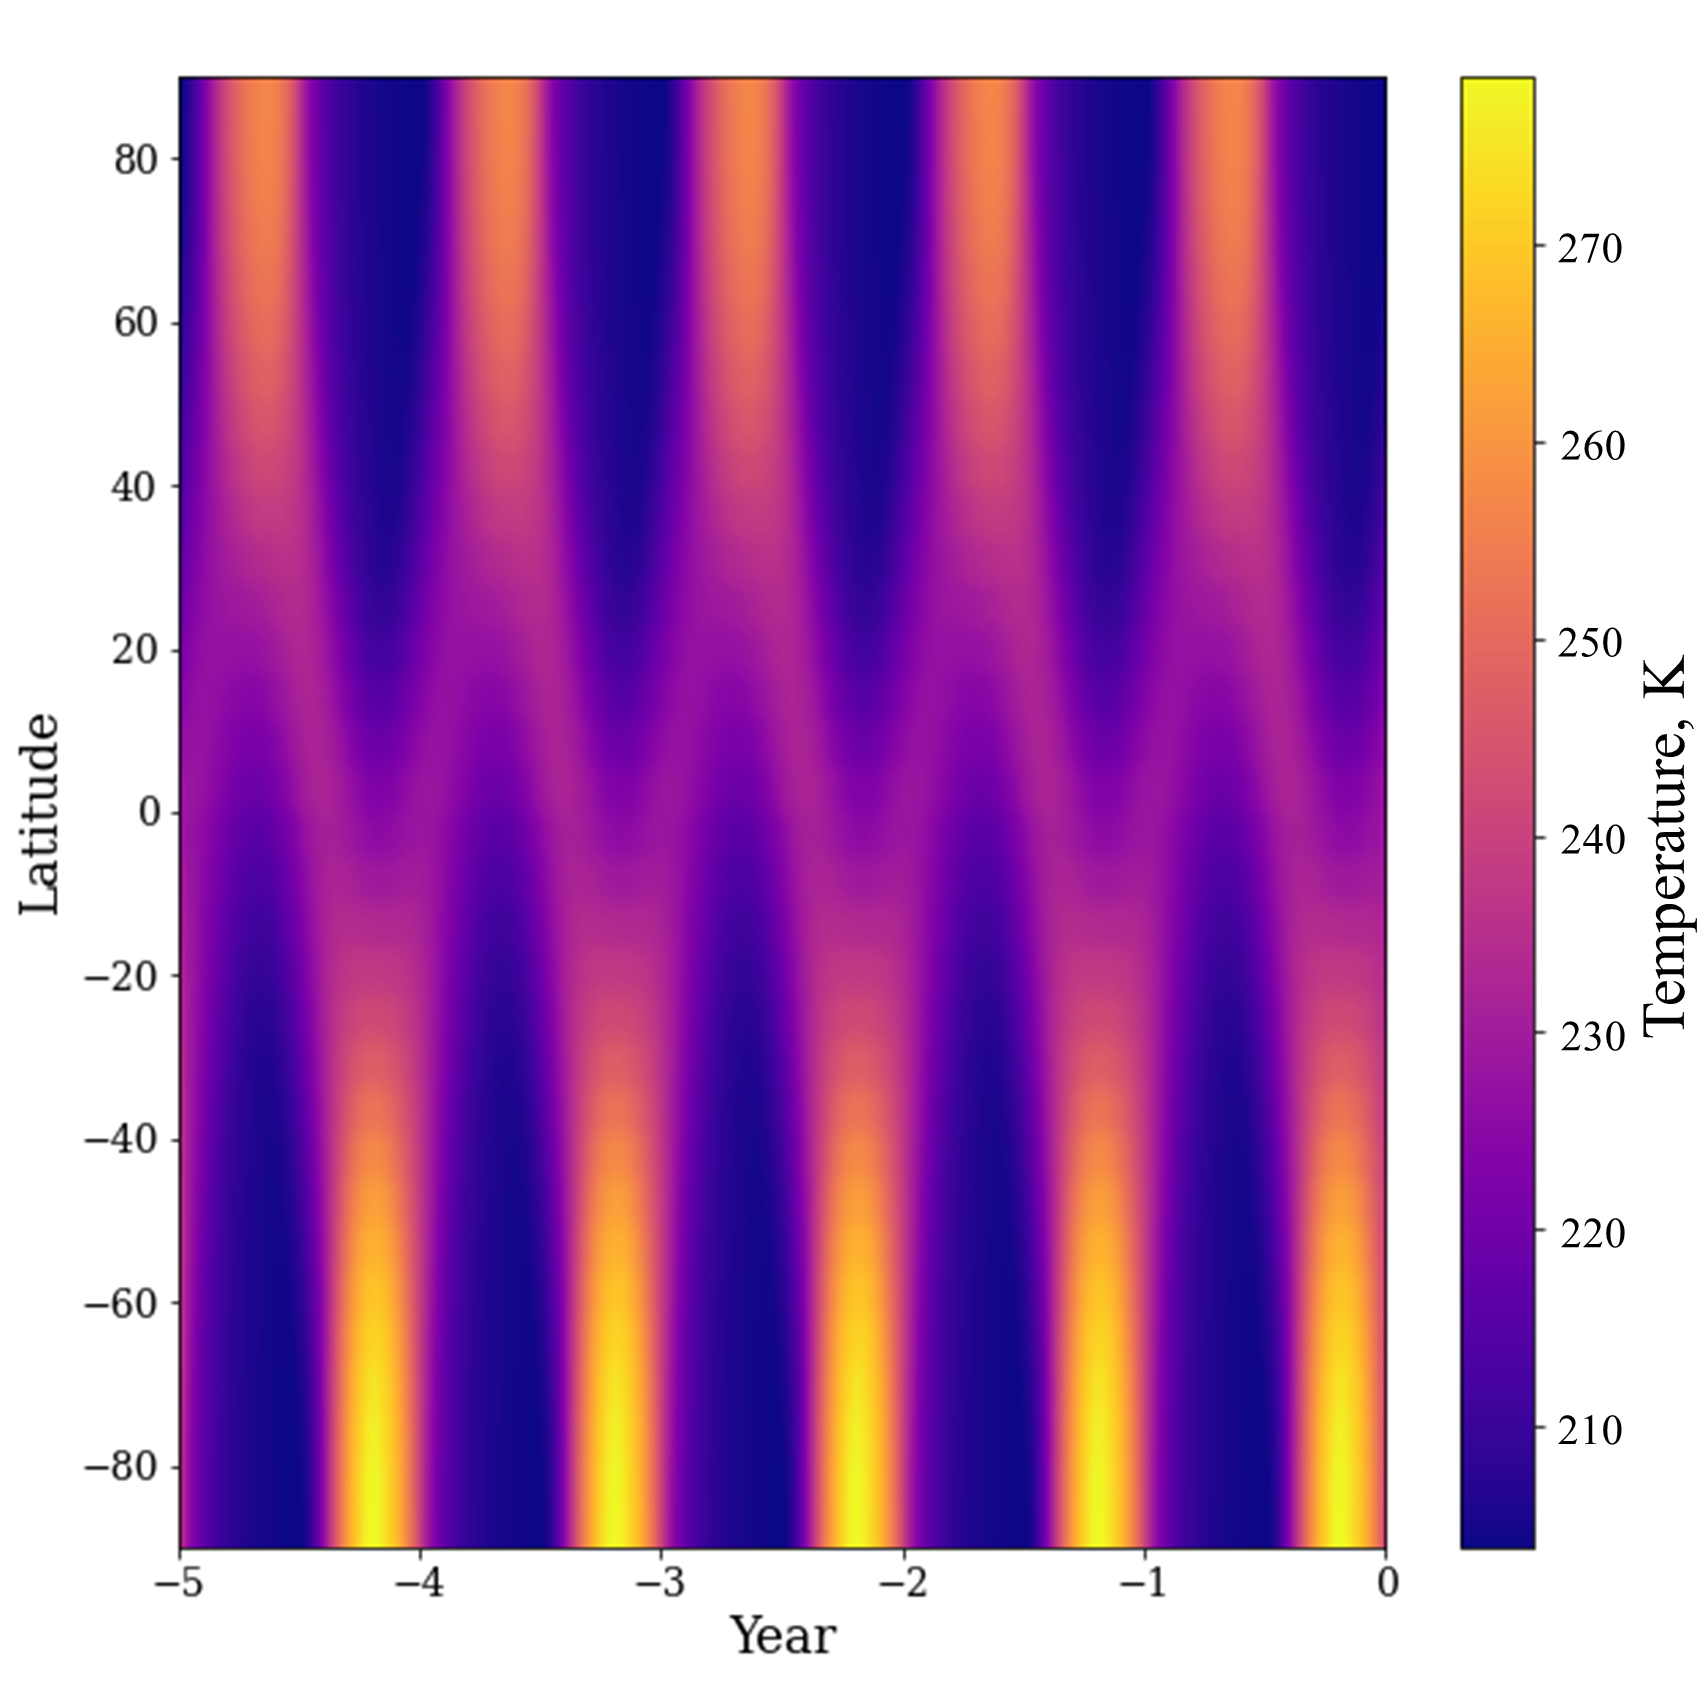
\includegraphics[width = 14cm]{ancient_mars_heatmap_new.png}
\caption{Heatmap displaying 5 Martian years of Ancient Mars' climate (Kelvin).}
\label{fig:ancientmars}
\end{figure}

\subsection{Limitations of the Ancient Mars Model}

The inverted temperature gradient observed in this models recreation of the ancient Martian climate is expected as a result of the high obliquity taken, however it is not representative of the behaviour expected of a hydrological cycle on Mars. Geological evidence for water is found across the globe, including the equator, near where the images in Fig. [X] were taken. 

\

As a result of temperatures consistently being above the condensation point of $\mathrm{CO_2}$, the model also predicts no surface carbon dioxide (and therefore no frozen poles) and no carbon dioxide cycle. 

\

It has been estimated that the largest losses of Mars' once-dense $\mathrm{CO_2}$ atmosphere were between 1-2 bars, as a result of solar-wind stripping and impact ejection, with remaining sinks such as surface carbonates and adsorbed gas accounting for no more than approximately 90 millibar of $\mathrm{CO_2}$ (a negligible amount) \cite{J19}. Therefore, while a 3.5 bar Martian atmosphere isn't entirely impossible - owing to uncertainty in how much $\mathrm{CO_2}$ is stored in deep carbon sinks - it is safe to say that such a dense atmosphere is incredibly improbable. Using more realistic estimates of the Martian atmosphere result in temperatures well below 273K. Further, even if 3.5 bar of $\mathrm{CO_2}$ were available and accessible to the atmosphere, dense atmospheres can result in adverse effects which counteract the greenhouse effect desired - these effects have been neglected in the parametrisation of outgoing infrared radiation in Eq. [X]. It has been argued that the condensation of $\mathrm{CO_2}$ in the atmosphere, resulting in clouds, would release latent heat and decrease the lapse rate - the rate at which temperature decreases with increasing altitude - and so decrease surface temperatures, to conserve energy balance \cite{K91}. $\mathrm{CO_2}$ clouds should also increase the planetary albedo, given that $\mathrm{CO_2}$ ice scatters effectively in the infrared, so the planet's surface receives less heat. Alternatively, it is possible that ice particles could induce infrared backscattering at a particular particle size ($\textgreater$ 10 $\mu$m) \cite{FP97}. The cooling or warming effects of $\mathrm{CO_2}$ clouds are not well-understood enough to comment on the expected effect of their inclusion in the model.

\

It should also be noted that the infrared outgoing radiation function described in Eq. [X] neglects the formation and effects of $\mathrm{H_2 O}$ clouds. This is a valid simplification at temperatures below the freezing point of water, but obviously not at temperatures above 273K, which the model does reach. $\mathrm{H_2 O}$ clouds similarly behave ambiguously, and their cooling or warming effect on the atmosphere is not well constrained. Cloud temperatures at low altitudes differ little from the temperature of the surface, so provide little greenhouse effect but contribute strongly to cloud cover albedo. High altitude clouds, conversely, produce a much stronger greenhouse effect than the effects of their albedo. Again, the net product of their inclusion cannot be commented on, especially as the ancient Martian atmosphere is not well known enough to constrain the altitudes of $\mathrm{H_2 O}$ clouds.

\

The ancient Mars solution somewhat resembles the 'icy highlands' hypothesis, proposed to describe the movement of ice on Mars. Areas of the planet receiving the lowest solar insolation become cold traps which retain ice deposits (as opposed to areas which, while they reach freezing point, will warm again and the water will migrate). At high obliquities, the movement of ice is equator-bound, which matches the equatorial temperature dips observed in the model. However, the model retains temperatures permanently above freezing point, and it is unlikely that even a warm and wet Mars would have a completely eliminated pressure cycle. There is a lack of evidence for glaciation during the Noachian era \cite{W16}, which seems to point in favour of a completely warm Mars with no ice caps - however, there should exist more evidence for glaciation regardless. Even if Mars did not have permanent or temporary ice caps during this period, at some point between now and then, temperatures have dropped low enough to form ice which would eventually become deposited in cold traps. 3D modelling investigating the icy highlands scenario indicates temperatures falling low enough for water ice to exist in highland valley networks located at the equator \cite{W12}.

\

All of the issues listed above could, theoretically, be accounted for in a much more comprehensive model. However, there remains a set of parameters that proves incredibly difficult to constrain - obliquity and eccentricity, due to their chaotic long-term and short-term variations. Both of these have been loosely constrained to between 0$\degree$ $\leq$ $\phi$ $\leq$ 60$\degree$ and 0 $\leq$ e $\leq$ 0.14 respectively, over the course of Mars' history \cite{L04}. Further back than 100Myr it becomes impossible to provide a precise evaluation of these values, given the chaotic nature of their evolution, so it is impossible to know exactly how this combination of parameters varied during the Noachian era (over 3.5Ga ago). It is certain, however, that the timescale of these variations - around 10$^5$ years for both obliquity and eccentricity - is much smaller than that of the Noachian era (~ 600Ga) and the minimum timescale over which valley networks are estimated to have formed (10$^5$ - 10$^7$) \cite{HHT11}. Mars would therefore have to have sustained temperatures above 273K over the full range of possible values for obliquity and eccentricity, and likely almost every parameter combination. This model, at its most extreme, predicts intermittent temperatures above freezing at only the South pole. Exploration of other parameter combinations returns stable solutions which are, on average, colder than this solution and spend less time above freezing.

\section{Potential for Future Work}

The EBM developed in this work is a relatively simple one, and certainly is simplified in comparison to higher dimensional EBMs and also GCMs. There remains potential for it to be further finetuned and built upon in order to achieve a more realistic picture of the ancient Martian climate. More importantly, building upon this model and others is necessary to continue the search for a viable warming mechanism for ancient Mars.
	
\
	
The next obvious possible solution to warm Mars is the inclusion of other, more potent, greenhouse gases in the model. While present-day Mars has an atmosphere consisting of almost entirely $\mathrm{CO_2}$, ancient Mars may have had a more diverse mix of gases in its atmosphere - methane, ammonia, and hydrogen have been named as potential Martian greenhouse gases. Any potential additional constituent would have to fill important windows in the absorption spectrum of $\mathrm{CO_2}$, particularly around the 400 cm$^{-1}$ and 1000 cm$^{-1}$ bands, to act as an additional effective greenhouse gas. Water vapour absorbs around these wavenumbers but is unlikely to produce the magnitude of warming required. The atmospheric concentration of water vapour is positively correlated with the temperature of the atmosphere, meaning that at low temperatures, the radiative forcing effect of $\mathrm{H_2O}$ on other greenhouse gases is minimal. Other gases, such as ammonia, have potential to absorb in important windows - but seem to have no formation method on Mars. Methane generates a strong greenhouse effect on Earth, however, its first significant absorption band is around 1300cm$^{-1}$, which is too far from the Planck function peak at colder Martian temperatures to provide the same magnitude of warming as on Earth. $\mathrm{CO_2}$-$\mathrm{H_2}$ absorption has also been explored as a warming mechanism, as it has been shown that $\mathrm{H_2}$ even in small quantities in an atmosphere can cause broadening of the absorption spectrum into window regions. This process would require a high rate of volcanic activity to supply the atmosphere with enough hydrogen, and a large atmospheric $\mathrm{CO_2}$ inventory, which might be inconsistent with the conditions expected of ancient Mars. As previously discussed, the effects of $\mathrm{CO_2}$ and $\mathrm{H_2O}$ clouds are uncertain at best. To summarise, the perfect greenhouse gas remains a mystery, but seems necessary for further warming.

\section{Concluding Remarks}

\begin{acknowledgments}
The author wishes to thank Drs. Richard Wilman and Craig Testrow for their insight and continuous commitment to the project, her parents for their never-ending support, her partner for all the encouragement, and her close friends for their camaraderie.
\end{acknowledgments}

%\bibliography{Draft1Notes}
\begin{thebibliography}{}

\bibitem{SMS08} D. Spiegel, K. Menou, C. Scharf., "Habitable Climates", The American Astronomical Society, vol. 681, 1609-1623 (2008). DOI: 
https://doi.org/10.1086/588089

\bibitem{WK97} D. Williams, J. Kasting., "Habitable Planets with High Obliquities", Icarus, vol. 129, 254-267 (1997). DOI: https://doi.org/10.1006/icar.1997.5759

\bibitem{AF89} J. Appelbaum, D. J. Flood., "Solar Radiation on Mars", Solar Energy, vol. 45, iss. 6, 353-363 (1990). DOI: https://doi.org/10.1016/0038-092X(90)90156-7

\bibitem{NC79} G. R. North, J. A. Coakley., "Differences between Seasonal and Mean Annual Energy Balance Model Calculations of Climate and Climate Sensitivity", Journal of the Atmospheric Sciences, vol. 36, 1189-1204 (1979). DOI: https://doi.org/10.1175/1520-0469(1979)036%3C1189:DBSAMA%3E2.0.CO;2

\bibitem{GQ01} P. R. Goode et al., "Earthshine Observations of the Earth's Reflectance", Geophysical Research Letters, vol. 28, 1671-1674 (2001). https://doi.org/10.1029/2000GL012580

\bibitem{PP12} D. K. Perovich, C. Polashenki., "Albedo evolution of seasonal Arctic sea ice", Geophysical Research Letters, vol. 39 (2012). DOI: https://doi.org/10.1029/2012GL051432

\bibitem{KH18} A. Kling, R. Haberle., "An analytical climate model to reproduce first order, yearly-averaged, climatology on early Mars: implications for the ancient lakes in the Gale crater", European Planetary Science Congress, vol. 12, 697 (2018). Bibcode: 2018EPSC...12..697K

\bibitem{FHT98} F. Forget, F. Hourdin, O. Talagrand., "$\mathrm{CO_2}$ Snowfall on Mars: Simulation with a General Circulation Model", Icarus, vol. 131, 302-316 (1998). DOI: https://doi.org/10.1006/icar.1997.5874

\bibitem{NT01} T. Nakamura, E. Tajika., "Stability and evolution of the climate system of Mars", Earth Planets Space, vol. 53, 851-859 (2001). DOI: 
https://doi.org/10.1186/BF03351682

\bibitem{CBZH} P. Ceppi et al., "Cloud feedback mechanisms and their representation in global climate models", Wiley Interdisciplinary Reviews. DOI: https://doi.org/10.1002/wcc.465

\bibitem{FP96} F. Forget, J. B. Pollack., "Thermal infrared observations of the condensing Martian polar caps: $\mathrm{CO_2}$ ice temperatures and radiative budget", Journal of Geophysical Research, vol. 101, 16865-16880 (1996). DOI: https://doi.org/10.1029/96JE01077

\bibitem{L20} G. Lohmann, "Temperatures from energy balance models: the effective heat capacity matters", European Geosciences Union, vol. 11, 1195-1208 (2020). DOI: 
https://doi.org/10.5194/esd-11-1195-2020

\bibitem{W16} R. D. Wordsworth, "The Climate of Early Mars", Annual Review of Earth \& Planetary Sciences, vol. 44, 1-31 (2016). DOI: https://doi.org/10.1146/annurev-earth-060115-012355

\bibitem{KS92} J. S. Kargel, R. G. Strom., "Ancient glaciation on Mars", Geological Society of America, vol. 20, 3-7 (1992). DOI: https://doi.org/10.1130/0091-7613(1992)020%3C0003:AGOM%3E2.3.CO;2

\bibitem{IPCC23} IPCC, 2023. \textit{Climate Change 2023: Synthesis Report,} [Core Writing Team, H. Lee and J. Romero]. IPCC, Geneva, Switzerland, 35-115. Available: https://www.ipcc.ch/report/sixth-assessment-report-cycle/

\bibitem{M14} V. Mastascusa \textit{et al.,} "Extremophiles Survival to Simulated Space Conditions: An Astrobiology Model Study", Origins of Life and Evolution of Biospheres, vol. 44, 231-237 (2014). DOI: https://doi.org/10.1007/s11084-014-9397-y

\bibitem{JN82} P. B. James, G. R. North., "The Seasonal $\mathrm{CO_2}$ Cycle on Mars: An Application of an Energy Balance Climate Model", Journal of Geophysical Research, vol. 87, 10271-10283 (1982). DOI: https://doi.org/10.1029/JB087iB12p10271

\bibitem{J19} B. M. Jakosky, "The $\mathrm{CO_2}$ inventory on Mars", Planetary and Space Science, vol. 175, 52-59 (2019). DOI: https://doi.org/10.1016/j.pss.2019.06.002

\bibitem{K23} G. Kopp, "Daily solar flux as a function of latitude and time", Solar Energy, vol. 249, 250-254 (2023). DOI: https://doi.org/10.1016/j.solener.2022.11.022

\bibitem{C13} J. Carter \textit{et al,} "Hydrous minerals on mars as seen
by the crism and omega imaging spectrometers: Updated global view", Journal of Geophysical
Research, vol. 118, 831–858 (2013). DOI: https://doi.org/10.1029/2012JE004145

\bibitem{EE14} B. L. Ehlmann, C. S. Edwards, "Mineralogy of the Martian surface", Annual Review of Earth and Planetary Sciences, vol. 42, 291-315 (2014). DOI: https://doi.org/10.1146/annurev-earth-060313-055024

\bibitem{JJ14} J. L. Fastook, J. W. Head, "Glaciation in the late noachian icy highlands: Ice accumulation,
distribution, flow rates, basal melting, and top-down melting rates and patterns", Planetary and
Space Science, vol. 106, 82-98 (2015). DOI: https://doi.org/10.1016/j.pss.2014.11.028

\bibitem{H54} \textit{Handbook of Chemistry and Physics}, 36th ed., Cleveland, Ohio, Chemical Rubber Publishing Co. 1954, 2239-2244.

\bibitem{FBSJS82} W. B. Banerdt \textit{et al.}, "Seasonal Carbon Dioxide Exchange Between the Regolith and Atmosphere of Mars: Experimental and Theoretical Studies", Journal of Geophysical Research, vol. 87, 10215-10225 (1982). DOI: https://doi.org/10.1029/JB087iB12p10215

\bibitem{K91} J. F. Kasting, "$\mathrm{CO_2}$ condensation and the climate of early Mars", Icarus, vol. 94, 1-13 (1991). DOI: https://doi.org/10.1016/0019-1035(91)90137-I

\bibitem{FP97} F. P. Forget, R. T. Pierrehumbert, "Warming early Mars with carbon dioxide clouds that scatter infrared radiation", Science, vol. 278, 1273-1276 (1997). DOI: https://doi.org/10.1126/science.278.5341.1273

\bibitem{K79} H. H. Kieffer, "Mars South Polar Spring and Summer Temperatures: A Residual $\mathrm{CO_2}$ Frost", Journal of Geophysical Research, vol. 84, 8263-8288 (1979). DOI: https://doi.org/10.1029/JB084iB14p08263

\bibitem{L04} Laskar \textit{et al.}, "Long term evolution and chaotic diffusion of the insolation qualities of Mars", Icarus, vol. 170 343-364 (2004). DOI: https://doi.org/10.1016/j.icarus.2004.04.005

\bibitem{HHT11} M. R. T. Hoke, B. M. Hynek, G. E. Tucker, "Formation timescales of large Martian valley networks", Earth and Planetary Science Letters, vol. 312, 1-12 (2011). DOI: https://doi.org/10.1016/j.epsl.2011.09.053

\bibitem{HBH10} B. M. Hynek, M. Beach, M. R. T. Hoke, "Updated global map of Martian valley networks and implications for climate and hydrologic processes", Journal of Geophysical Research, vol. 115, E09008 (2010). DOI: https://doi.org/10.1029/2009JE003548

\bibitem{H24} A. Harri \textit{et al.}, "Perseverance MEDA Atmospheric Pressure Observations - Initial Results", JGR Planets, vol. 129, iss. 3 (2024). DOI: https://doi.org/10.1029/2023JE007880

\bibitem{WR15} H. Wang, M. I. Richardson, "The origin, evolution, and trajectory of large dust storms on Mars during Mars years 24-30 (1999-2011)", Icarus, vol. 251, 112-127 (2015). DOI: https://doi.org/10.1016/j.icarus.2013.10.033

\bibitem{K76} H. H. Kieffer, "Soil and Surface Temperatures at the Viking Landing Sites", Science, vol. 194, iss. 4271, 1344-1346 (1976). DOI: https://doi.org/10.1126/science.194.4271.1344

\bibitem{M01} J. P. Merrison \textit{et al.}, "The Mars Simulation Laboratory", in First European Workshop on Exo/Astrobiology, Frascati, Italy, 2001, p. 371-374. Bibcode: 2001ESASP.496..371M 

\bibitem{S04} S. E. Smrekar \textit{et al.}, "Geologic evolution of the Martian dichotomy in the Ismenius area of Mars and implications for plains magnetisation", Journal of Geophysical Research, vol. 109, iss. E11 (2004). DOI: https://doi.org/10.1029/2004JE002260

\bibitem{WR13} H. Wang, M. I. Richardson, "The origin, evolution, and trajectory of large dust storms on Mars during Mars years 24-30 (199-2011)", Icarus, vol. 251, p 112-127 (2015). DOI: http://dx.doi.org/10.1016/j.icarus.2013.10.033

\bibitem{W20} Z. Wu \textit{et al.}, "Dust tides and rapid meridional motions in the Martian atmosphere during major dust storms", Nature Communications, vol. 11, article 614 (2020). DOI: https://doi.org/10.1038/s41467-020-14510-x

\bibitem{HKP02} J. W. Head, M. A. Kreslavsky, S. Pratt, "Northern lowlands of Mars: Evidence for widespread volcanic flooding and tectonic deformation in the Hesperian Period", Journal of Geophysical Research (Planets), vol. 107, iss. E1 (2002). DOI: https://doi.org/10.1029/2000JE001445

\bibitem{HZS07}
I. Halevy, M. T. Zuber, D. P. Schrag, "A sulfur dioxide climate feedback on early Mars", Science, vol. 318, p. 1903-1907 (2007). DOI: https://doi.org/10.1126/science.1147039

\bibitem{HH14} I. Halevy, J. W. Head, "Episodic warming of early Mars by punctuated volcanism", Nature Geoscience, vol. 7, p. 865-868 (2014). DOI: 
https://doi.org/10.1038/ngeo2293

\bibitem{FH08} C. I. Fassett, J. W. Head, "The timing of martian valley network activity: Constraints from buffered crater counting", Icarus, vol. 195, iss. 1, pp. 61-89 (2008). DOI:  https://doi.org/10.1016/j.icarus.2007.12.009

\bibitem{H99} J. W. Head \textit{et al.}, "Possible ancient oceans on Mars: evidence from Mars Orbiter Laser Altimeter data", Science, vol 286, pp. 2134-2137 (1999). DOI: https://doi.org/10.1126/science.286.5447.2134

\bibitem{W13} R. M. E. Williams \textit{et al.}, "Martian fluvial conglomerates at gale crater", Science, vol. 340, iss. 6136, pp. 1068-1072 (2013). DOI: https://doi.org/10.1126/science.1237317

\bibitem{BHM09} C. J. Barnhart, A. D. Howard, J. M. Moore, "Long-term precipitation and late-stage valley network formation: Landform simulations of Parana Basin, Mars", Journal of Geophysical Research (Atmospheres), vol. 114 (2009). DOI: http://dx.doi.org/10.1029/2008JE003122

\bibitem{E11} B. L. Ehlmann \textit{et al.}, "Subsurface water and clay mineral formation during the early history of Mars", Nature, vol. 479, pp. 53-60 (2011). DOI: https://doi.org/10.1038/nature10582

\bibitem{G81} D. O. Gough, "Solar interior structure and luminosity variations", Solar Physics, vol. 74, pp. 21-34 (1981). DOI: 
https://doi.org/10.1007/BF00151270

\bibitem{MM07} D. A. Minton, R. Malhotra, "Assessing the massive young sun hypothesis to solve the warm young earth puzzle", The Astrophysical Journal, vol. 660, pp. 1700-1706 (2007). DOI: https://doi.org/10.1086/514331

\bibitem{W12} R. Wordsworth \textit{et al.}, "Global modelling of the early martian climate under a denser CO2 atmosphere: Water cycle and ice evolution", Icarus, vol. 222, iss. 1, pp. 1-19 (2013). DOI: https://doi.org/10.1016/j.icarus.2012.09.036

\end{thebibliography} 

\newpage
 
\section{Summary for a General Audience}
\clearpage

\newpage

\section{Appendices}
\subsection{Appendix A: convergence and stability testing}

\begin{figure}[H]
%\centering
\begin{subfigure}{.5\textwidth}
  \centering
  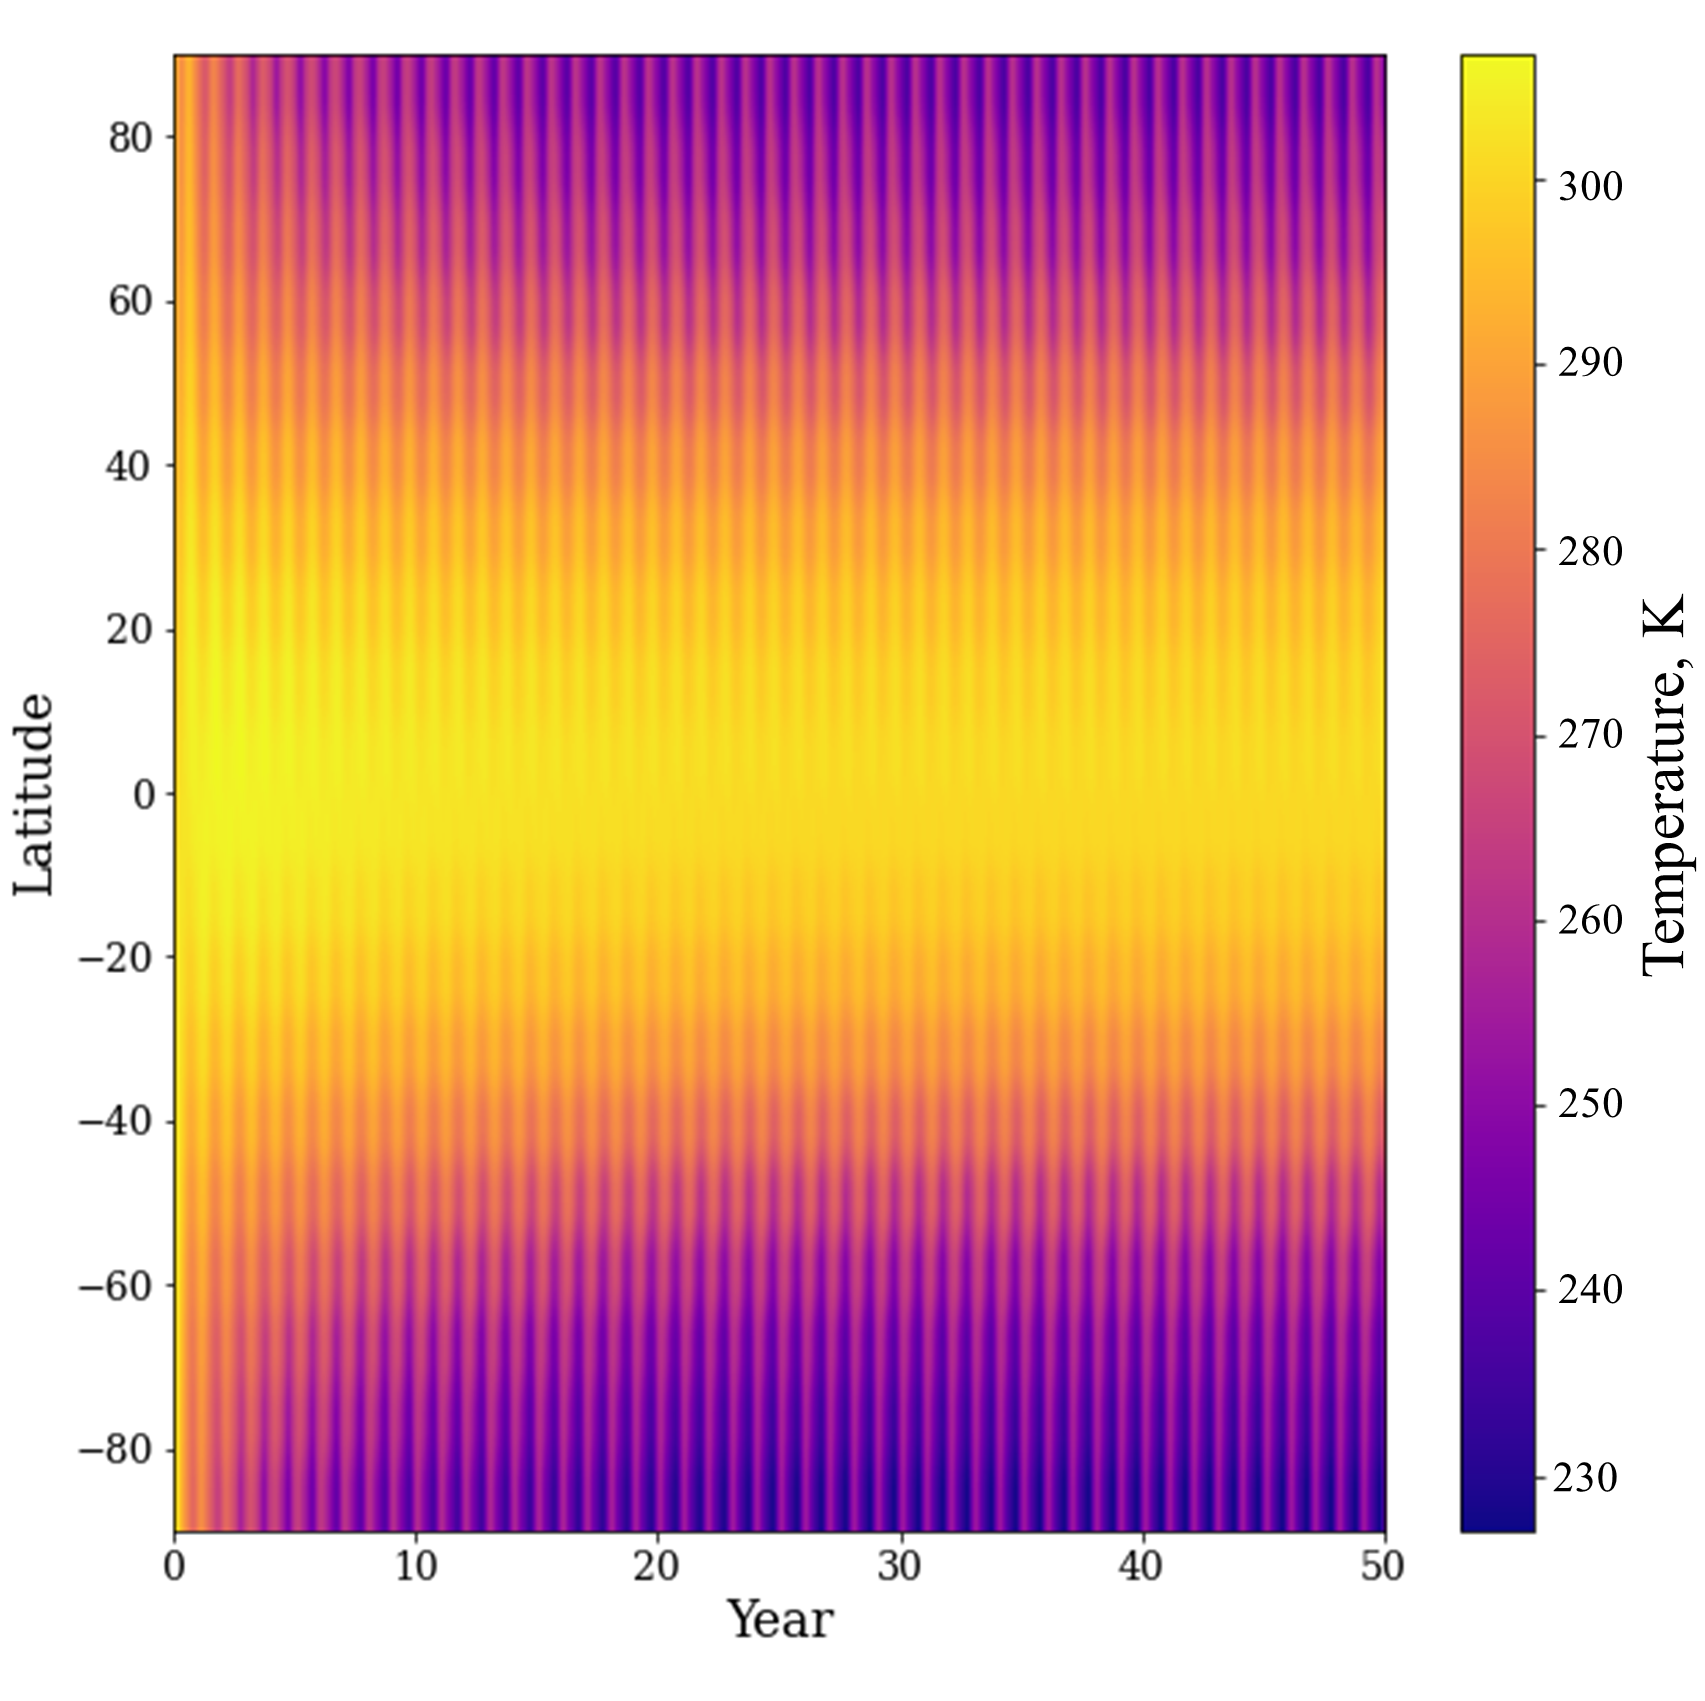
\includegraphics[width = 8cm]{Earth50yrsHeatmapNew.png}
  \caption{Heatmap of Earth climate between 0 - 50 years}
  \label{fig:sub1}
\end{subfigure}%
\begin{subfigure}{.5\textwidth}
  \centering
  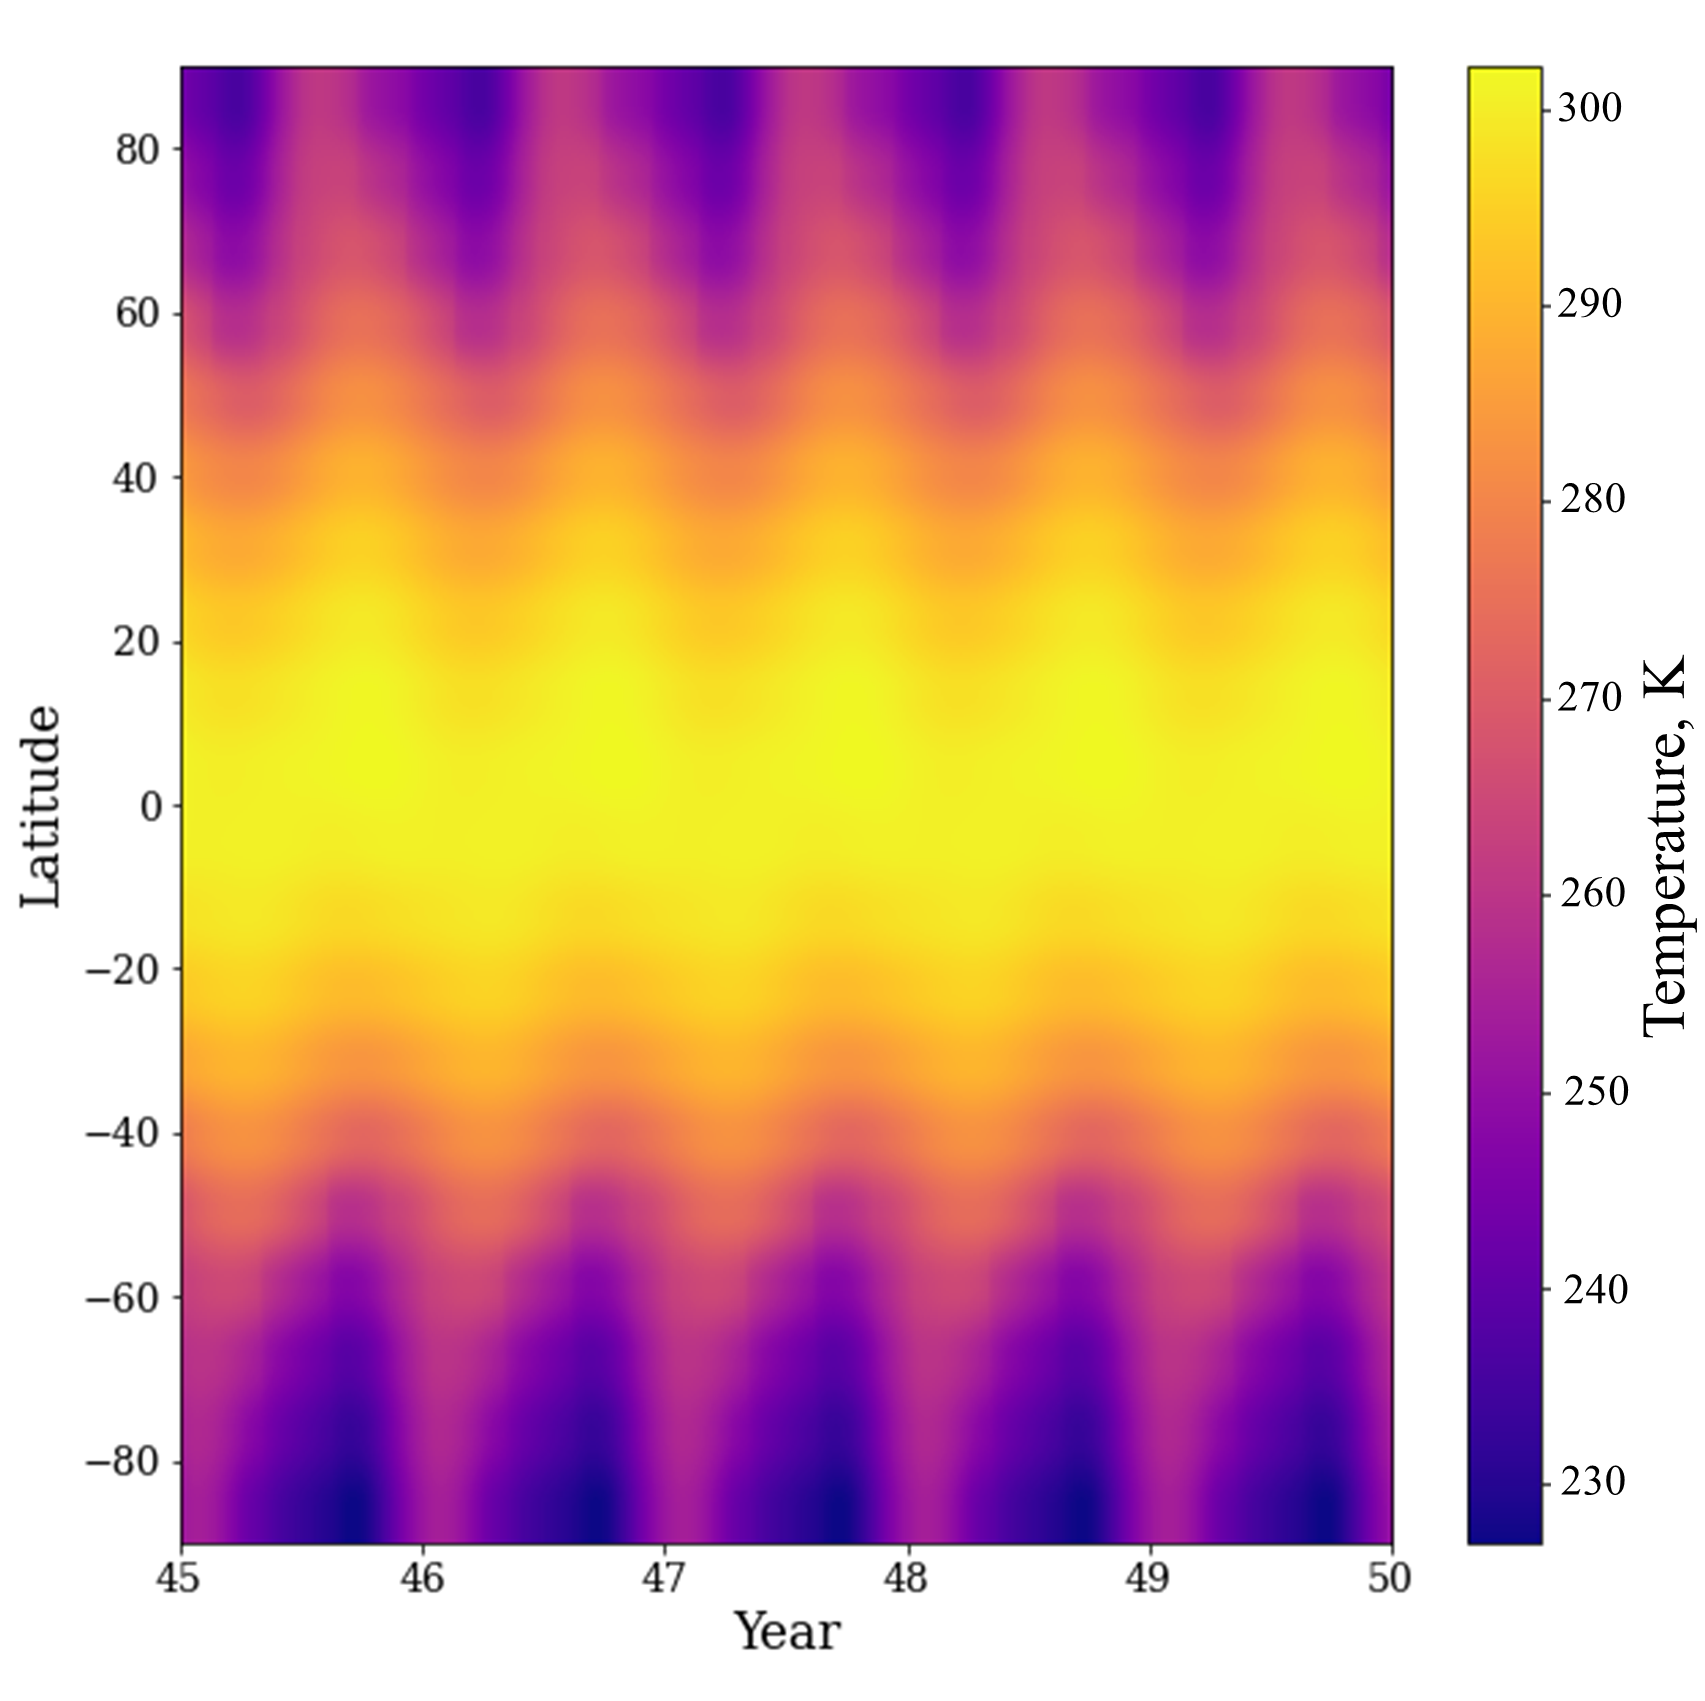
\includegraphics[width=8cm]{Earth5yrsHeatmapNew.png}
  \caption{Heatmap of Earth climate last 5 years of modelling}
  \label{fig:sub2}
\end{subfigure}
\raggedright
\caption{Heatmaps displaying Earth's climate (Kelvin) 50 years post model initialisation. Full heatmap (a) displays temperatures plotted every 73 days, settled heatmap (b) shows temperatures plotted every 5 days. Negative latitudes (degrees) correspond to the Southern hemisphere.}
\label{fig:test}
\end{figure}

\begin{figure}[H]
%\centering
\begin{subfigure}{.5\textwidth}
  \centering
  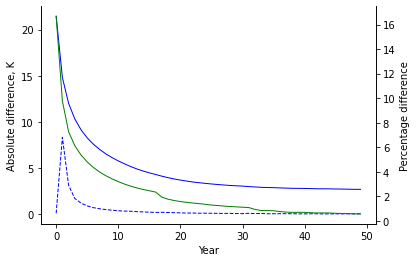
\includegraphics[width = 8cm]{Convergence.png}
  \caption{Earth convergence tests}
  \label{fig:sub1}
\end{subfigure}%
\begin{subfigure}{.5\textwidth}
  \centering
  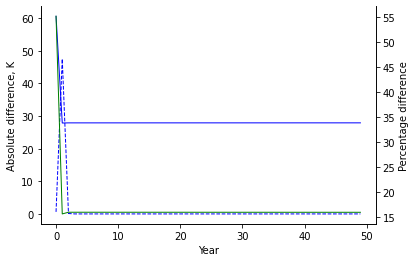
\includegraphics[width=8cm]{MarsConvergence.png}
  \caption{Mars convergence tests}
  \label{fig:sub2}
\end{subfigure}
\raggedright
\caption{Convergence tests for both planet models. Blue tests indicate comparison to empirical models Eqs. X by absolute (solid line) and percentage (dashed line) difference. Green test shows change in temperature compared to same time last year, $\delta$ = $|T_{year} - T_{year-1}|$. The average difference is taken at the Southern summer solstice.}
\label{fig:test}
\end{figure}

\newpage

\subsection{Appendix B: the finite difference method}

Below are the expressions used to describe the differential terms in Eq. X, alongside the code used to implement them. Boundary conditions are applied since no heat will diffuse further than the poles latitudinally, which simplify the expressions for the North and South poles. 

\begin{verbatim}
def temp_difference(index): 
	d = diffusion(pressure_mars)
    if index != 0 and index != n-1: #most latitudes
        ir, a = outgoing_2(index)
        second_order_term = d*(temps[index+1] - 2*temps[index] 
        + temps[index-1])/(del_lamb**2)
        first_order_term = -d*np.tan(lats[index])*((temps[index+1] 
        - temps[index-1])/(2*del_lamb))
        rad_term = solar[index][day]*(1-a) - ir
        
        temp_diff[index] = (second_order_term + first_order_term 
        + rad_term)*(del_t/heatcap(cl))
        
    elif index == 0: #south pole
        ir, a = outgoing_2(0)
        second_order_term = d*((temps[0+1] - temps[0])/del_lamb**2)
        rad_term = solar[0][day]*(1-a) - ir

        temp_diff[0] = (second_order_term + rad_term)
        *(del_t/heatcap(cl))

    elif index == n-1: #north pole
        ir, a = outgoing_2(n-1)
        second_order_term = -d*((temps[-1] - temps[-1-1])/del_lamb**2)
        rad_term = solar[n-1][day]*(1-a) - ir

        temp_diff[-1] = (second_order_term + rad_term)
        *(del_t/heatcap(cl))

    return temp_diff
\end{verbatim}

Here \verb|index| refers to the latitude band in a list and \verb|n| to the total number of nodes, \verb|ir, a| refer to the outgoing radiation and albedo terms respectively (both of which are outputs of the temperature-dependent \verb|outgoing_2| function), and \verb|solar[index][day]| therefore refers to the flux received by latitude \verb|index| on a particular day. Additionally, \verb|d| refers to the diffusion coefficient and \verb|heatcap(cl)| to the heat capacity at this band (temperature dependent).

\end{document}
